\documentclass{article}
\usepackage{amsmath}
\usepackage{color,pxfonts,fix-cm}
\usepackage{latexsym}
\usepackage[mathletters]{ucs}
\DeclareUnicodeCharacter{8211}{\textendash}
\DeclareUnicodeCharacter{8212}{\textemdash}
\DeclareUnicodeCharacter{46}{\textperiodcentered}
\DeclareUnicodeCharacter{58}{$\colon$}
\DeclareUnicodeCharacter{124}{\textbar}
\DeclareUnicodeCharacter{8226}{$\bullet$}
\DeclareUnicodeCharacter{8764}{$\sim$}
\usepackage[T1]{fontenc}
\usepackage[utf8x]{inputenc}
\usepackage{pict2e}
\usepackage{wasysym}
\usepackage[english]{babel}
\usepackage{tikz}
\pagestyle{empty}
\usepackage[margin=0in,paperwidth=595pt,paperheight=841pt]{geometry}
\begin{document}
\definecolor{color_31474}{rgb}{0,0.2,0.4}
\definecolor{color_33132}{rgb}{0,0.4,0.701961}
\definecolor{color_283006}{rgb}{1,1,1}
\definecolor{color_109231}{rgb}{0.313726,0.313726,0.313726}
\definecolor{color_29791}{rgb}{0,0,0}
\definecolor{color_33759}{rgb}{0,0.501961,0}
\definecolor{color_214303}{rgb}{0.752941,0,0}
\definecolor{color_277561}{rgb}{0.980392,0.921569,0.921569}
\definecolor{color_273076}{rgb}{0.960784,0.960784,0.960784}
\definecolor{color_279186}{rgb}{1,0.54902,0}
\definecolor{color_178741}{rgb}{0.588235,0.588235,0.588235}
\definecolor{color_268210}{rgb}{0.941177,0.952941,0.964706}
\begin{tikzpicture}[overlay]
\path(0pt,0pt);
\filldraw[color_31474][nonzero rule]
(-15.00134pt, 10.89111pt) -- (-15.00134pt, -130.843pt)
 -- (-15.00134pt, -130.843pt)
 -- (580.2819pt, -130.843pt)
 -- (580.2819pt, -130.843pt)
 -- (580.2819pt, 10.89111pt) -- cycle
;
\filldraw[color_33132][nonzero rule]
(-15.00134pt, -102.4962pt) -- (-15.00134pt, -159.1898pt)
 -- (-15.00134pt, -159.1898pt)
 -- (580.2819pt, -159.1898pt)
 -- (580.2819pt, -159.1898pt)
 -- (580.2819pt, -102.4962pt) -- cycle
;
\end{tikzpicture}
\begin{picture}(-5,0)(2.5,0)
\put(150.499,-124.786){\fontsize{11.9552}{1}\usefont{T1}{cmr}{b}{n}\selectfont\color{color_283006}BANQUE NATIONALE DE MAURITANIE}
\put(211.408,-144.004){\fontsize{9.9626}{1}\usefont{T1}{cmr}{m}{n}\selectfont\color{color_283006}Direction Système d'Information}
\put(190.571,-270.723){\fontsize{29.7484}{1}\usefont{T1}{cmr}{b}{n}\selectfont\color{color_31474}Blueprint DR}
\put(119.09,-295.886){\fontsize{14.3462}{1}\usefont{T1}{cmr}{m}{n}\selectfont\color{color_109231}Disaster Recovery — Architecture \& Plan d'Exécution}
\put(143.347,-375.587){\fontsize{10.9091}{1}\usefont{T1}{cmr}{b}{n}\selectfont\color{color_31474}Version}
\put(223.015,-375.587){\fontsize{10.9091}{1}\usefont{T1}{cmr}{m}{n}\selectfont\color{color_29791}1.0}
\put(143.347,-392.125){\fontsize{10.9091}{1}\usefont{T1}{cmr}{b}{n}\selectfont\color{color_31474}Date}
\put(223.014,-392.125){\fontsize{10.9091}{1}\usefont{T1}{cmr}{m}{n}\selectfont\color{color_29791}22 Mars 2026}
\put(143.347,-408.663){\fontsize{10.9091}{1}\usefont{T1}{cmr}{b}{n}\selectfont\color{color_31474}Statut}
\put(223.0063,-408.663){\fontsize{10.9091}{1}\usefont{T1}{cmr}{b}{n}\selectfont\color{color_33759}Actif — Document de Référence}
\put(143.347,-425.201){\fontsize{10.9091}{1}\usefont{T1}{cmr}{b}{n}\selectfont\color{color_31474}Go-Live}
\put(223.0074,-425.201){\fontsize{10.9091}{1}\usefont{T1}{cmr}{b}{n}\selectfont\color{color_214303}fin Avril 2026}
\put(143.347,-441.739){\fontsize{10.9091}{1}\usefont{T1}{cmr}{b}{n}\selectfont\color{color_31474}Titulaires}
\put(223.0074,-441.739){\fontsize{10.9091}{1}\usefont{T1}{cmr}{m}{n}\selectfont\color{color_29791}Ing. Betah lab \& Dr. Fatimetou abdou}
\put(143.347,-458.277){\fontsize{10.9091}{1}\usefont{T1}{cmr}{b}{n}\selectfont\color{color_31474}Stagiaires}
\put(223.014,-458.277){\fontsize{10.9091}{1}\usefont{T1}{cmr}{m}{n}\selectfont\color{color_29791}Ethmane Mahmoud Ethmane, Ahmed abd Dayem Ahmed Bouha}
\put(143.347,-474.815){\fontsize{10.9091}{1}\usefont{T1}{cmr}{b}{n}\selectfont\color{color_31474}Direction}
\put(223.014,-474.815){\fontsize{10.9091}{1}\usefont{T1}{cmr}{m}{n}\selectfont\color{color_29791}Direction Système d'Information — BNM}
\put(56.12598,-746.242){\fontsize{9.9626}{1}\usefont{T1}{cmr}{m}{n}\selectfont\color{color_109231}Document de référence unique du projet DR. Toute modification validée par le Team Lead uniquement.}
\end{picture}
\newpage
\begin{tikzpicture}[overlay]\path(0pt,0pt);\end{tikzpicture}
\begin{picture}(-5,0)(2.5,0)
\put(41.693,-31.48297){\fontsize{9.9626}{1}\usefont{T1}{cmr}{b}{n}\selectfont\color{color_31474}BNM}
\put(150.0482,-31.48297){\fontsize{9.9626}{1}\usefont{T1}{cmr}{m}{n}\selectfont\color{color_109231}}
\put(348.1446,-31.48297){\fontsize{9.9626}{1}\usefont{T1}{cmr}{m}{n}\selectfont\color{color_109231}Blueprin t DR v1.0 — CONFIDENTIEL}
\end{picture}
\begin{tikzpicture}[overlay]
\path(0pt,0pt);
\draw[color_29791,line width=0.398pt]
(41.693pt, -35.26898pt) -- (523.583pt, -35.26898pt)
;
\end{tikzpicture}
\begin{picture}(-5,0)(2.5,0)
\put(41.693,-70.935){\fontsize{11.9552}{1}\usefont{T1}{cmr}{b}{n}\selectfont\color{color_31474}Con ten ts}
\end{picture}
\begin{tikzpicture}[overlay]
\path(0pt,0pt);
\draw[color_31474,line width=0.797pt]
(41.693pt, -77.51099pt) -- (523.583pt, -77.51099pt)
;
\end{tikzpicture}
\begin{picture}(-5,0)(2.5,0)
\put(41.693,-106.247){\fontsize{10.9091}{1}\usefont{T1}{cmr}{b}{n}\selectfont\color{color_29791}1 Con texte et Ob jectifs 3}
\put(41.693,-130.644){\fontsize{10.9091}{1}\usefont{T1}{cmr}{b}{n}\selectfont\color{color_29791}2 Equip e et Resp onsabilités 3}
\put(41.693,-155.04){\fontsize{10.9091}{1}\usefont{T1}{cmr}{b}{n}\selectfont\color{color_29791}3 In v en taire Pro duction — Zone 0 3}
\put(41.693,-179.437){\fontsize{10.9091}{1}\usefont{T1}{cmr}{b}{n}\selectfont\color{color_29791}4 Arc hitec t u re DR Choisie 3}
\put(57.964,-192.986){\fontsize{10.9091}{1}\usefont{T1}{cmr}{m}{n}\selectfont\color{color_29791}4.1}
\put(496.31,-192.986){\fontsize{10.9091}{1}\usefont{T1}{cmr}{m}{n}\selectfont\color{color_29791}}
\put(518.1609,-192.986){\fontsize{10.9091}{1}\usefont{T1}{cmr}{m}{n}\selectfont\color{color_29791}4}
\put(57.964,-206.535){\fontsize{10.9091}{1}\usefont{T1}{cmr}{m}{n}\selectfont\color{color_29791}4.2}
\put(496.3056,-206.535){\fontsize{10.9091}{1}\usefont{T1}{cmr}{m}{n}\selectfont\color{color_29791}}
\put(518.1566,-206.535){\fontsize{10.9091}{1}\usefont{T1}{cmr}{m}{n}\selectfont\color{color_29791}4}
\put(57.964,-220.084){\fontsize{10.9091}{1}\usefont{T1}{cmr}{m}{n}\selectfont\color{color_29791}4.3}
\put(496.3045,-220.084){\fontsize{10.9091}{1}\usefont{T1}{cmr}{m}{n}\selectfont\color{color_29791}}
\put(518.1555,-220.084){\fontsize{10.9091}{1}\usefont{T1}{cmr}{m}{n}\selectfont\color{color_29791}4}
\put(41.693,-244.481){\fontsize{10.9091}{1}\usefont{T1}{cmr}{b}{n}\selectfont\color{color_29791}5 Ob jectifs R TO / RPO 5}
\put(41.693,-268.877){\fontsize{10.9091}{1}\usefont{T1}{cmr}{b}{n}\selectfont\color{color_29791}6 Infrastructure — Une VM pa r Zone 5}
\put(41.693,-293.2729){\fontsize{10.9091}{1}\usefont{T1}{cmr}{b}{n}\selectfont\color{color_29791}7 Plan d’Exécution 5}
\put(57.96402,-306.8229){\fontsize{10.9091}{1}\usefont{T1}{cmr}{m}{n}\selectfont\color{color_29791}7.1}
\put(496.3002,-306.8229){\fontsize{10.9091}{1}\usefont{T1}{cmr}{m}{n}\selectfont\color{color_29791}}
\put(518.162,-306.8229){\fontsize{10.9091}{1}\usefont{T1}{cmr}{m}{n}\selectfont\color{color_29791}5}
\put(41.69302,-331.2189){\fontsize{10.9091}{1}\usefont{T1}{cmr}{b}{n}\selectfont\color{color_29791}8 P oin ts Ouv erts 6}
\put(41.69302,-355.6149){\fontsize{10.9091}{1}\usefont{T1}{cmr}{b}{n}\selectfont\color{color_29791}9 Con trôle du Do cumen t 6}
\end{picture}
\begin{tikzpicture}[overlay]
\path(0pt,0pt);
\draw[color_29791,line width=0.398pt]
(41.693pt, -777.389pt) -- (523.583pt, -777.389pt)
;
\end{tikzpicture}
\begin{picture}(-5,0)(2.5,0)
\put(271.848,-790.022){\fontsize{9.9626}{1}\usefont{T1}{cmr}{m}{n}\selectfont\color{color_109231}2}
\put(293.424,-790.022){\fontsize{9.9626}{1}\usefont{T1}{cmr}{m}{n}\selectfont\color{color_109231}}
\put(407.2965,-790.022){\fontsize{9.9626}{1}\usefont{T1}{cmr}{m}{n}\selectfont\color{color_109231}Usage In terne Uniquemen t}
\end{picture}
\newpage
\begin{tikzpicture}[overlay]\path(0pt,0pt);\end{tikzpicture}
\begin{picture}(-5,0)(2.5,0)
\put(41.693,-31.48297){\fontsize{9.9626}{1}\usefont{T1}{cmr}{b}{n}\selectfont\color{color_31474}BNM}
\put(150.0482,-31.48297){\fontsize{9.9626}{1}\usefont{T1}{cmr}{m}{n}\selectfont\color{color_109231}}
\put(348.1446,-31.48297){\fontsize{9.9626}{1}\usefont{T1}{cmr}{m}{n}\selectfont\color{color_109231}Blueprin t DR v1.0 — CONFIDENTIEL}
\end{picture}
\begin{tikzpicture}[overlay]
\path(0pt,0pt);
\draw[color_29791,line width=0.398pt]
(41.693pt, -35.26898pt) -- (523.583pt, -35.26898pt)
;
\end{tikzpicture}
\begin{picture}(-5,0)(2.5,0)
\put(41.693,-70.935){\fontsize{11.9552}{1}\usefont{T1}{cmr}{b}{n}\selectfont\color{color_31474}1}
\put(48.41661,-70.935){\fontsize{11.9552}{1}\usefont{T1}{cmr}{b}{n}\selectfont\color{color_31474}}
\put(61.86621,-70.935){\fontsize{11.9552}{1}\usefont{T1}{cmr}{b}{n}\selectfont\color{color_31474}Con texte et Ob jectifs}
\end{picture}
\begin{tikzpicture}[overlay]
\path(0pt,0pt);
\draw[color_31474,line width=0.797pt]
(41.693pt, -77.51099pt) -- (523.583pt, -77.51099pt)
;
\filldraw[color_214303][nonzero rule]
(41.693pt, -139.634pt) -- (42.889pt, -139.634pt)
 -- (42.889pt, -139.634pt)
 -- (42.889pt, -87.87097pt)
 -- (42.889pt, -87.87097pt)
 -- (41.693pt, -87.87097pt) -- cycle
;
\filldraw[color_214303][nonzero rule]
(42.888pt, -89.06702pt) -- (522.387pt, -89.06702pt)
 -- (522.387pt, -89.06702pt)
 -- (522.387pt, -87.87103pt)
 -- (522.387pt, -87.87103pt)
 -- (42.888pt, -87.87103pt) -- cycle
;
\filldraw[color_277561][nonzero rule]
(42.888pt, -139.634pt) -- (522.387pt, -139.634pt)
 -- (522.387pt, -139.634pt)
 -- (522.387pt, -89.06696pt)
 -- (522.387pt, -89.06696pt)
 -- (42.888pt, -89.06696pt) -- cycle
;
\filldraw[color_214303][nonzero rule]
(41.693pt, -140.83pt) -- (523.583pt, -140.83pt)
 -- (523.583pt, -140.83pt)
 -- (523.583pt, -139.634pt)
 -- (523.583pt, -139.634pt)
 -- (41.693pt, -139.634pt) -- cycle
;
\filldraw[color_214303][nonzero rule]
(522.387pt, -139.634pt) -- (523.583pt, -139.634pt)
 -- (523.583pt, -139.634pt)
 -- (523.583pt, -87.87097pt)
 -- (523.583pt, -87.87097pt)
 -- (522.387pt, -87.87097pt) -- cycle
;
\end{tikzpicture}
\begin{picture}(-5,0)(2.5,0)
\put(52.851,-104.566){\fontsize{10.9091}{1}\usefont{T1}{cmr}{b}{n}\selectfont\color{color_214303}Situation}
\put(151.142,-104.566){\fontsize{10.9091}{1}\usefont{T1}{cmr}{m}{n}\selectfont\color{color_29791}}
\put(154.2184,-104.566){\fontsize{10.9091}{1}\usefont{T1}{cmr}{m}{n}\selectfont\color{color_29791}— Aucune stratégie de sauv egarde ou de reprise après sinistre n’ est actuelle-}
\put(52.851,-118.115){\fontsize{10.9091}{1}\usefont{T1}{cmr}{m}{n}\selectfont\color{color_29791}men}
\put(343.1094,-118.115){\fontsize{10.9091}{1}\usefont{T1}{cmr}{b}{n}\selectfont\color{color_29791}}
\put(346.7967,-118.115){\fontsize{10.9091}{1}\usefont{T1}{cmr}{b}{n}\selectfont\color{color_29791}p erte totale et irrév ersible des}
\put(52.851,-131.664){\fontsize{10.9091}{1}\usefont{T1}{cmr}{b}{n}\selectfont\color{color_29791}données .}
\put(58.629,-157.325){\fontsize{10.9091}{1}\usefont{T1}{cmr}{b}{n}\selectfont\color{color_29791}Ob}
\put(115.2232,-157.325){\fontsize{10.9091}{1}\usefont{T1}{cmr}{m}{n}\selectfont\color{color_29791}}
\put(120.0123,-157.325){\fontsize{10.9091}{1}\usefont{T1}{cmr}{m}{n}\selectfont\color{color_29791}Zéro p erte de données sur les bases critiques via ré plication sync hrone, infrastructure}
\put(41.693,-170.874){\fontsize{10.9091}{1}\usefont{T1}{cmr}{m}{n}\selectfont\color{color_29791}résilien}
\put(373.118,-170.874){\fontsize{10.9091}{1}\usefont{T1}{cmr}{b}{n}\selectfont\color{color_29791}}
\put(376.7398,-170.874){\fontsize{10.9091}{1}\usefont{T1}{cmr}{b}{n}\selectfont\color{color_29791}fin Avril 2026 .}
\end{picture}
\begin{tikzpicture}[overlay]
\path(0pt,0pt);
\draw[color_29791,line width=0.398pt]
(41.693pt, -186.145pt) -- (523.583pt, -186.145pt)
;
\draw[color_29791,line width=0.398pt]
(41.892pt, -199.894pt) -- (41.892pt, -186.345pt)
;
\filldraw[color_31474][nonzero rule]
(42.091pt, -199.894pt) -- (123.519pt, -199.894pt)
 -- (123.519pt, -199.894pt)
 -- (123.519pt, -186.345pt)
 -- (123.519pt, -186.345pt)
 -- (42.091pt, -186.345pt) -- cycle
;
\end{tikzpicture}
\begin{picture}(-5,0)(2.5,0)
\put(48.069,-195.829){\fontsize{10.9091}{1}\usefont{T1}{cmr}{b}{n}\selectfont\color{color_283006}Système}
\end{picture}
\begin{tikzpicture}[overlay]
\path(0pt,0pt);
\draw[color_29791,line width=0.398pt]
(123.719pt, -199.894pt) -- (123.719pt, -186.345pt)
;
\filldraw[color_31474][nonzero rule]
(123.918pt, -199.894pt) -- (191.527pt, -199.894pt)
 -- (191.527pt, -199.894pt)
 -- (191.527pt, -186.345pt)
 -- (191.527pt, -186.345pt)
 -- (123.918pt, -186.345pt) -- cycle
;
\end{tikzpicture}
\begin{picture}(-5,0)(2.5,0)
\put(129.896,-195.829){\fontsize{10.9091}{1}\usefont{T1}{cmr}{b}{n}\selectfont\color{color_283006}T yp e}
\end{picture}
\begin{tikzpicture}[overlay]
\path(0pt,0pt);
\draw[color_29791,line width=0.398pt]
(191.726pt, -199.894pt) -- (191.726pt, -186.345pt)
;
\filldraw[color_31474][nonzero rule]
(191.925pt, -199.894pt) -- (454.854pt, -199.894pt)
 -- (454.854pt, -199.894pt)
 -- (454.854pt, -186.345pt)
 -- (454.854pt, -186.345pt)
 -- (191.925pt, -186.345pt) -- cycle
;
\end{tikzpicture}
\begin{picture}(-5,0)(2.5,0)
\put(197.903,-195.829){\fontsize{10.9091}{1}\usefont{T1}{cmr}{b}{n}\selectfont\color{color_283006}Description}
\end{picture}
\begin{tikzpicture}[overlay]
\path(0pt,0pt);
\draw[color_29791,line width=0.398pt]
(455.054pt, -199.894pt) -- (455.054pt, -186.345pt)
;
\filldraw[color_31474][nonzero rule]
(455.253pt, -199.894pt) -- (523.184pt, -199.894pt)
 -- (523.184pt, -199.894pt)
 -- (523.184pt, -186.345pt)
 -- (523.184pt, -186.345pt)
 -- (455.253pt, -186.345pt) -- cycle
;
\end{tikzpicture}
\begin{picture}(-5,0)(2.5,0)
\put(461.23,-195.829){\fontsize{10.9091}{1}\usefont{T1}{cmr}{b}{n}\selectfont\color{color_283006}Criticité}
\end{picture}
\begin{tikzpicture}[overlay]
\path(0pt,0pt);
\draw[color_29791,line width=0.398pt]
(523.383pt, -199.894pt) -- (523.383pt, -186.345pt)
;
\draw[color_29791,line width=0.398pt]
(41.693pt, -200.093pt) -- (523.583pt, -200.093pt)
;
\draw[color_29791,line width=0.398pt]
(41.892pt, -213.841pt) -- (41.892pt, -200.292pt)
;
\end{tikzpicture}
\begin{picture}(-5,0)(2.5,0)
\put(48.069,-209.777){\fontsize{10.9091}{1}\usefont{T1}{cmr}{b}{n}\selectfont\color{color_29791}Monétique}
\end{picture}
\begin{tikzpicture}[overlay]
\path(0pt,0pt);
\draw[color_29791,line width=0.398pt]
(123.719pt, -213.841pt) -- (123.719pt, -200.292pt)
;
\end{tikzpicture}
\begin{picture}(-5,0)(2.5,0)
\put(129.896,-209.777){\fontsize{10.9091}{1}\usefont{T1}{cmr}{m}{n}\selectfont\color{color_29791}Oracle 19c}
\end{picture}
\begin{tikzpicture}[overlay]
\path(0pt,0pt);
\draw[color_29791,line width=0.398pt]
(191.726pt, -213.841pt) -- (191.726pt, -200.292pt)
;
\end{tikzpicture}
\begin{picture}(-5,0)(2.5,0)
\put(197.903,-209.777){\fontsize{10.9091}{1}\usefont{T1}{cmr}{m}{n}\selectfont\color{color_29791}T raitemen t des paiemen ts}
\end{picture}
\begin{tikzpicture}[overlay]
\path(0pt,0pt);
\draw[color_29791,line width=0.398pt]
(455.054pt, -213.841pt) -- (455.054pt, -200.292pt)
;
\end{tikzpicture}
\begin{picture}(-5,0)(2.5,0)
\put(461.23,-209.777){\fontsize{10.9091}{1}\usefont{T1}{cmr}{b}{n}\selectfont\color{color_214303}Critique}
\end{picture}
\begin{tikzpicture}[overlay]
\path(0pt,0pt);
\draw[color_29791,line width=0.398pt]
(523.383pt, -213.841pt) -- (523.383pt, -200.292pt)
;
\draw[color_29791,line width=0.398pt]
(41.693pt, -214.041pt) -- (523.583pt, -214.041pt)
;
\draw[color_29791,line width=0.398pt]
(41.892pt, -227.789pt) -- (41.892pt, -214.24pt)
;
\filldraw[color_273076][nonzero rule]
(42.091pt, -227.789pt) -- (123.519pt, -227.789pt)
 -- (123.519pt, -227.789pt)
 -- (123.519pt, -214.24pt)
 -- (123.519pt, -214.24pt)
 -- (42.091pt, -214.24pt) -- cycle
;
\end{tikzpicture}
\begin{picture}(-5,0)(2.5,0)
\put(48.069,-223.724){\fontsize{10.9091}{1}\usefont{T1}{cmr}{b}{n}\selectfont\color{color_29791}Clic k}
\end{picture}
\begin{tikzpicture}[overlay]
\path(0pt,0pt);
\draw[color_29791,line width=0.398pt]
(123.719pt, -227.789pt) -- (123.719pt, -214.24pt)
;
\filldraw[color_273076][nonzero rule]
(123.918pt, -227.789pt) -- (191.527pt, -227.789pt)
 -- (191.527pt, -227.789pt)
 -- (191.527pt, -214.24pt)
 -- (191.527pt, -214.24pt)
 -- (123.918pt, -214.24pt) -- cycle
;
\end{tikzpicture}
\begin{picture}(-5,0)(2.5,0)
\put(129.896,-223.724){\fontsize{10.9091}{1}\usefont{T1}{cmr}{m}{n}\selectfont\color{color_29791}MySQL 8.0}
\end{picture}
\begin{tikzpicture}[overlay]
\path(0pt,0pt);
\draw[color_29791,line width=0.398pt]
(191.726pt, -227.789pt) -- (191.726pt, -214.24pt)
;
\filldraw[color_273076][nonzero rule]
(191.925pt, -227.789pt) -- (454.854pt, -227.789pt)
 -- (454.854pt, -227.789pt)
 -- (454.854pt, -214.24pt)
 -- (454.854pt, -214.24pt)
 -- (191.925pt, -214.24pt) -- cycle
;
\end{tikzpicture}
\begin{picture}(-5,0)(2.5,0)
\put(197.903,-223.724){\fontsize{10.9091}{1}\usefont{T1}{cmr}{m}{n}\selectfont\color{color_29791}P ortefeuille et paiemen ts mobil es}
\end{picture}
\begin{tikzpicture}[overlay]
\path(0pt,0pt);
\draw[color_29791,line width=0.398pt]
(455.054pt, -227.789pt) -- (455.054pt, -214.24pt)
;
\filldraw[color_273076][nonzero rule]
(455.253pt, -227.789pt) -- (523.184pt, -227.789pt)
 -- (523.184pt, -227.789pt)
 -- (523.184pt, -214.24pt)
 -- (523.184pt, -214.24pt)
 -- (455.253pt, -214.24pt) -- cycle
;
\end{tikzpicture}
\begin{picture}(-5,0)(2.5,0)
\put(461.23,-223.724){\fontsize{10.9091}{1}\usefont{T1}{cmr}{b}{n}\selectfont\color{color_214303}Critique}
\end{picture}
\begin{tikzpicture}[overlay]
\path(0pt,0pt);
\draw[color_29791,line width=0.398pt]
(523.383pt, -227.789pt) -- (523.383pt, -214.24pt)
;
\draw[color_29791,line width=0.398pt]
(41.693pt, -227.988pt) -- (523.583pt, -227.988pt)
;
\draw[color_29791,line width=0.398pt]
(41.892pt, -241.737pt) -- (41.892pt, -228.188pt)
;
\end{tikzpicture}
\begin{picture}(-5,0)(2.5,0)
\put(48.069,-237.672){\fontsize{10.9091}{1}\usefont{T1}{cmr}{b}{n}\selectfont\color{color_29791}Pleniged DB}
\end{picture}
\begin{tikzpicture}[overlay]
\path(0pt,0pt);
\draw[color_29791,line width=0.398pt]
(123.719pt, -241.737pt) -- (123.719pt, -228.188pt)
;
\end{tikzpicture}
\begin{picture}(-5,0)(2.5,0)
\put(129.896,-237.672){\fontsize{10.9091}{1}\usefont{T1}{cmr}{m}{n}\selectfont\color{color_29791}MySQL 8.0}
\end{picture}
\begin{tikzpicture}[overlay]
\path(0pt,0pt);
\draw[color_29791,line width=0.398pt]
(191.726pt, -241.737pt) -- (191.726pt, -228.188pt)
;
\end{tikzpicture}
\begin{picture}(-5,0)(2.5,0)
\put(197.903,-237.672){\fontsize{10.9091}{1}\usefont{T1}{cmr}{m}{n}\selectfont\color{color_29791}Arc hiv age do cumen taire}
\end{picture}
\begin{tikzpicture}[overlay]
\path(0pt,0pt);
\draw[color_29791,line width=0.398pt]
(455.054pt, -241.737pt) -- (455.054pt, -228.188pt)
;
\end{tikzpicture}
\begin{picture}(-5,0)(2.5,0)
\put(461.23,-237.672){\fontsize{10.9091}{1}\usefont{T1}{cmr}{b}{n}\selectfont\color{color_214303}Critique}
\end{picture}
\begin{tikzpicture}[overlay]
\path(0pt,0pt);
\draw[color_29791,line width=0.398pt]
(523.383pt, -241.737pt) -- (523.383pt, -228.188pt)
;
\draw[color_29791,line width=0.398pt]
(41.693pt, -241.936pt) -- (523.583pt, -241.936pt)
;
\draw[color_29791,line width=0.398pt]
(41.892pt, -255.684pt) -- (41.892pt, -242.135pt)
;
\filldraw[color_273076][nonzero rule]
(42.091pt, -255.684pt) -- (123.519pt, -255.684pt)
 -- (123.519pt, -255.684pt)
 -- (123.519pt, -242.135pt)
 -- (123.519pt, -242.135pt)
 -- (42.091pt, -242.135pt) -- cycle
;
\end{tikzpicture}
\begin{picture}(-5,0)(2.5,0)
\put(48.069,-251.62){\fontsize{10.9091}{1}\usefont{T1}{cmr}{b}{n}\selectfont\color{color_29791}Pleniged FS}
\end{picture}
\begin{tikzpicture}[overlay]
\path(0pt,0pt);
\draw[color_29791,line width=0.398pt]
(123.719pt, -255.684pt) -- (123.719pt, -242.135pt)
;
\filldraw[color_273076][nonzero rule]
(123.918pt, -255.684pt) -- (191.527pt, -255.684pt)
 -- (191.527pt, -255.684pt)
 -- (191.527pt, -242.135pt)
 -- (191.527pt, -242.135pt)
 -- (123.918pt, -242.135pt) -- cycle
;
\end{tikzpicture}
\begin{picture}(-5,0)(2.5,0)
\put(129.896,-251.62){\fontsize{10.9091}{1}\usefont{T1}{cmr}{m}{n}\selectfont\color{color_29791}File System}
\end{picture}
\begin{tikzpicture}[overlay]
\path(0pt,0pt);
\draw[color_29791,line width=0.398pt]
(191.726pt, -255.684pt) -- (191.726pt, -242.135pt)
;
\filldraw[color_273076][nonzero rule]
(191.925pt, -255.684pt) -- (454.854pt, -255.684pt)
 -- (454.854pt, -255.684pt)
 -- (454.854pt, -242.135pt)
 -- (454.854pt, -242.135pt)
 -- (191.925pt, -242.135pt) -- cycle
;
\end{tikzpicture}
\begin{picture}(-5,0)(2.5,0)
\put(197.903,-251.62){\fontsize{10.9091}{1}\usefont{T1}{cmr}{m}{n}\selectfont\color{color_29791}Images et PDF s ( ∼ 4 TB)}
\end{picture}
\begin{tikzpicture}[overlay]
\path(0pt,0pt);
\draw[color_29791,line width=0.398pt]
(455.054pt, -255.684pt) -- (455.054pt, -242.135pt)
;
\filldraw[color_273076][nonzero rule]
(455.253pt, -255.684pt) -- (523.184pt, -255.684pt)
 -- (523.184pt, -255.684pt)
 -- (523.184pt, -242.135pt)
 -- (523.184pt, -242.135pt)
 -- (455.253pt, -242.135pt) -- cycle
;
\end{tikzpicture}
\begin{picture}(-5,0)(2.5,0)
\put(461.23,-251.62){\fontsize{10.9091}{1}\usefont{T1}{cmr}{b}{n}\selectfont\color{color_279186}Imp ortan t}
\end{picture}
\begin{tikzpicture}[overlay]
\path(0pt,0pt);
\draw[color_29791,line width=0.398pt]
(523.383pt, -255.684pt) -- (523.383pt, -242.135pt)
;
\draw[color_29791,line width=0.398pt]
(41.693pt, -255.884pt) -- (523.583pt, -255.884pt)
;
\end{tikzpicture}
\begin{picture}(-5,0)(2.5,0)
\put(214.01,-280.591){\fontsize{10.9091}{1}\usefont{T1}{cmr}{m}{n}\selectfont\color{color_29791}T able 1: P érimètre du pro jet}
\put(41.69299,-310.607){\fontsize{11.9552}{1}\usefont{T1}{cmr}{b}{n}\selectfont\color{color_31474}2}
\put(48.4166,-310.607){\fontsize{11.9552}{1}\usefont{T1}{cmr}{b}{n}\selectfont\color{color_31474}}
\put(61.8662,-310.607){\fontsize{11.9552}{1}\usefont{T1}{cmr}{b}{n}\selectfont\color{color_31474}Equip e et Resp onsabilités}
\end{picture}
\begin{tikzpicture}[overlay]
\path(0pt,0pt);
\draw[color_31474,line width=0.797pt]
(41.693pt, -317.182pt) -- (523.583pt, -317.182pt)
;
\draw[color_29791,line width=0.398pt]
(41.693pt, -339.698pt) -- (523.583pt, -339.698pt)
;
\draw[color_29791,line width=0.398pt]
(41.892pt, -353.446pt) -- (41.892pt, -339.897pt)
;
\filldraw[color_31474][nonzero rule]
(42.091pt, -353.446pt) -- (114.137pt, -353.446pt)
 -- (114.137pt, -353.446pt)
 -- (114.137pt, -339.897pt)
 -- (114.137pt, -339.897pt)
 -- (42.091pt, -339.897pt) -- cycle
;
\end{tikzpicture}
\begin{picture}(-5,0)(2.5,0)
\put(48.069,-349.382){\fontsize{10.9091}{1}\usefont{T1}{cmr}{b}{n}\selectfont\color{color_283006}Rôle}
\end{picture}
\begin{tikzpicture}[overlay]
\path(0pt,0pt);
\draw[color_29791,line width=0.398pt]
(114.337pt, -353.446pt) -- (114.337pt, -339.897pt)
;
\filldraw[color_31474][nonzero rule]
(114.536pt, -353.446pt) -- (293.699pt, -353.446pt)
 -- (293.699pt, -353.446pt)
 -- (293.699pt, -339.897pt)
 -- (293.699pt, -339.897pt)
 -- (114.536pt, -339.897pt) -- cycle
;
\end{tikzpicture}
\begin{picture}(-5,0)(2.5,0)
\put(120.513,-349.382){\fontsize{10.9091}{1}\usefont{T1}{cmr}{b}{n}\selectfont\color{color_283006}Nom}
\end{picture}
\begin{tikzpicture}[overlay]
\path(0pt,0pt);
\draw[color_29791,line width=0.398pt]
(293.898pt, -353.446pt) -- (293.898pt, -339.897pt)
;
\filldraw[color_31474][nonzero rule]
(294.097pt, -353.446pt) -- (523.184pt, -353.446pt)
 -- (523.184pt, -353.446pt)
 -- (523.184pt, -339.897pt)
 -- (523.184pt, -339.897pt)
 -- (294.097pt, -339.897pt) -- cycle
;
\end{tikzpicture}
\begin{picture}(-5,0)(2.5,0)
\put(300.075,-349.382){\fontsize{10.9091}{1}\usefont{T1}{cmr}{b}{n}\selectfont\color{color_283006}Resp onsabilités}
\end{picture}
\begin{tikzpicture}[overlay]
\path(0pt,0pt);
\draw[color_29791,line width=0.398pt]
(523.383pt, -353.446pt) -- (523.383pt, -339.897pt)
;
\draw[color_29791,line width=0.398pt]
(41.693pt, -353.646pt) -- (523.583pt, -353.646pt)
;
\draw[color_29791,line width=0.398pt]
(41.892pt, -367.394pt) -- (41.892pt, -353.845pt)
;
\end{tikzpicture}
\begin{picture}(-5,0)(2.5,0)
\put(48.069,-363.329){\fontsize{10.9091}{1}\usefont{T1}{cmr}{b}{n}\selectfont\color{color_29791}Direction}
\end{picture}
\begin{tikzpicture}[overlay]
\path(0pt,0pt);
\draw[color_29791,line width=0.398pt]
(114.337pt, -367.394pt) -- (114.337pt, -353.845pt)
;
\end{tikzpicture}
\begin{picture}(-5,0)(2.5,0)
\put(120.513,-363.329){\fontsize{10.9091}{1}\usefont{T1}{cmr}{m}{n}\selectfont\color{color_29791}Direction SI — BNM}
\end{picture}
\begin{tikzpicture}[overlay]
\path(0pt,0pt);
\draw[color_29791,line width=0.398pt]
(293.898pt, -367.394pt) -- (293.898pt, -353.845pt)
;
\end{tikzpicture}
\begin{picture}(-5,0)(2.5,0)
\put(300.075,-363.329){\fontsize{10.9091}{1}\usefont{T1}{cmr}{m}{n}\selectfont\color{color_29791}Sup ervision, v alidation, resso urces}
\end{picture}
\begin{tikzpicture}[overlay]
\path(0pt,0pt);
\draw[color_29791,line width=0.398pt]
(523.383pt, -367.394pt) -- (523.383pt, -353.845pt)
;
\draw[color_29791,line width=0.398pt]
(41.693pt, -367.593pt) -- (523.583pt, -367.593pt)
;
\draw[color_29791,line width=0.398pt]
(41.892pt, -394.891pt) -- (41.892pt, -367.793pt)
;
\filldraw[color_273076][nonzero rule]
(42.091pt, -394.891pt) -- (114.137pt, -394.891pt)
 -- (114.137pt, -394.891pt)
 -- (114.137pt, -367.793pt)
 -- (114.137pt, -367.793pt)
 -- (42.091pt, -367.793pt) -- cycle
;
\end{tikzpicture}
\begin{picture}(-5,0)(2.5,0)
\put(48.069,-377.277){\fontsize{10.9091}{1}\usefont{T1}{cmr}{b}{n}\selectfont\color{color_29791}T eam Lead}
\end{picture}
\begin{tikzpicture}[overlay]
\path(0pt,0pt);
\draw[color_29791,line width=0.398pt]
(114.337pt, -394.891pt) -- (114.337pt, -367.793pt)
;
\filldraw[color_273076][nonzero rule]
(114.536pt, -394.891pt) -- (293.699pt, -394.891pt)
 -- (293.699pt, -394.891pt)
 -- (293.699pt, -367.793pt)
 -- (293.699pt, -367.793pt)
 -- (114.536pt, -367.793pt) -- cycle
;
\end{tikzpicture}
\begin{picture}(-5,0)(2.5,0)
\put(124.13,-377.277){\fontsize{10.9091}{1}\usefont{T1}{cmr}{m}{n}\selectfont\color{color_29791}Betah L a b (Titulaire: Fatimateau Abdou)}
\end{picture}
\begin{tikzpicture}[overlay]
\path(0pt,0pt);
\draw[color_29791,line width=0.398pt]
(293.898pt, -394.891pt) -- (293.898pt, -367.793pt)
;
\filldraw[color_273076][nonzero rule]
(294.097pt, -394.891pt) -- (523.184pt, -394.891pt)
 -- (523.184pt, -394.891pt)
 -- (523.184pt, -367.793pt)
 -- (523.184pt, -367.793pt)
 -- (294.097pt, -367.793pt) -- cycle
;
\end{tikzpicture}
\begin{picture}(-5,0)(2.5,0)
\put(300.075,-377.277){\fontsize{10.9091}{1}\usefont{T1}{cmr}{m}{n}\selectfont\color{color_29791}Arc hitecture, pilot age, DR v alidation, rep ort-}
\put(300.075,-390.826){\fontsize{10.9091}{1}\usefont{T1}{cmr}{m}{n}\selectfont\color{color_29791}ing, Jira}
\end{picture}
\begin{tikzpicture}[overlay]
\path(0pt,0pt);
\draw[color_29791,line width=0.398pt]
(523.383pt, -394.891pt) -- (523.383pt, -367.793pt)
;
\draw[color_29791,line width=0.398pt]
(41.693pt, -395.09pt) -- (523.583pt, -395.09pt)
;
\draw[color_29791,line width=0.398pt]
(41.892pt, -422.388pt) -- (41.892pt, -395.29pt)
;
\end{tikzpicture}
\begin{picture}(-5,0)(2.5,0)
\put(48.069,-404.774){\fontsize{10.9091}{1}\usefont{T1}{cmr}{b}{n}\selectfont\color{color_29791}Ingénieur}
\end{picture}
\begin{tikzpicture}[overlay]
\path(0pt,0pt);
\draw[color_29791,line width=0.398pt]
(114.337pt, -422.388pt) -- (114.337pt, -395.29pt)
;
\end{tikzpicture}
\begin{picture}(-5,0)(2.5,0)
\put(124.13,-404.774){\fontsize{10.9091}{1}\usefont{T1}{cmr}{m}{n}\selectfont\color{color_29791}Boulery ah EL Hedrami}
\end{picture}
\begin{tikzpicture}[overlay]
\path(0pt,0pt);
\draw[color_29791,line width=0.398pt]
(293.898pt, -422.388pt) -- (293.898pt, -395.29pt)
;
\end{tikzpicture}
\begin{picture}(-5,0)(2.5,0)
\put(300.075,-404.774){\fontsize{10.9091}{1}\usefont{T1}{cmr}{m}{n}\selectfont\color{color_29791}Sup ervision tec hnique, v alidati on des tra v a ux,}
\put(300.075,-418.323){\fontsize{10.9091}{1}\usefont{T1}{cmr}{m}{n}\selectfont\color{color_29791}supp ort stagiaires}
\end{picture}
\begin{tikzpicture}[overlay]
\path(0pt,0pt);
\draw[color_29791,line width=0.398pt]
(523.383pt, -422.388pt) -- (523.383pt, -395.29pt)
;
\draw[color_29791,line width=0.398pt]
(41.693pt, -422.587pt) -- (523.583pt, -422.587pt)
;
\draw[color_29791,line width=0.398pt]
(41.892pt, -449.885pt) -- (41.892pt, -422.787pt)
;
\filldraw[color_273076][nonzero rule]
(42.091pt, -449.885pt) -- (114.137pt, -449.885pt)
 -- (114.137pt, -449.885pt)
 -- (114.137pt, -422.787pt)
 -- (114.137pt, -422.787pt)
 -- (42.091pt, -422.787pt) -- cycle
;
\end{tikzpicture}
\begin{picture}(-5,0)(2.5,0)
\put(48.069,-432.271){\fontsize{10.9091}{1}\usefont{T1}{cmr}{b}{n}\selectfont\color{color_29791}Stagiaire 1}
\end{picture}
\begin{tikzpicture}[overlay]
\path(0pt,0pt);
\draw[color_29791,line width=0.398pt]
(114.337pt, -449.885pt) -- (114.337pt, -422.787pt)
;
\filldraw[color_273076][nonzero rule]
(114.536pt, -449.885pt) -- (293.699pt, -449.885pt)
 -- (293.699pt, -449.885pt)
 -- (293.699pt, -422.787pt)
 -- (293.699pt, -422.787pt)
 -- (114.536pt, -422.787pt) -- cycle
;
\end{tikzpicture}
\begin{picture}(-5,0)(2.5,0)
\put(124.13,-432.271){\fontsize{10.9091}{1}\usefont{T1}{cmr}{m}{n}\selectfont\color{color_29791}Ethmane Mahmoud Ethmane}
\end{picture}
\begin{tikzpicture}[overlay]
\path(0pt,0pt);
\draw[color_29791,line width=0.398pt]
(293.898pt, -449.885pt) -- (293.898pt, -422.787pt)
;
\filldraw[color_273076][nonzero rule]
(294.097pt, -449.885pt) -- (523.184pt, -449.885pt)
 -- (523.184pt, -449.885pt)
 -- (523.184pt, -422.787pt)
 -- (523.184pt, -422.787pt)
 -- (294.097pt, -422.787pt) -- cycle
;
\end{tikzpicture}
\begin{picture}(-5,0)(2.5,0)
\put(300.075,-432.271){\fontsize{10.9091}{1}\usefont{T1}{cmr}{m}{n}\selectfont\color{color_29791}T rac k Oracle — Monétique (Data Guard,}
\put(300.075,-445.82){\fontsize{10.9091}{1}\usefont{T1}{cmr}{m}{n}\selectfont\color{color_29791}RMAN)}
\end{picture}
\begin{tikzpicture}[overlay]
\path(0pt,0pt);
\draw[color_29791,line width=0.398pt]
(523.383pt, -449.885pt) -- (523.383pt, -422.787pt)
;
\draw[color_29791,line width=0.398pt]
(41.693pt, -450.084pt) -- (523.583pt, -450.084pt)
;
\draw[color_29791,line width=0.398pt]
(41.892pt, -477.382pt) -- (41.892pt, -450.284pt)
;
\end{tikzpicture}
\begin{picture}(-5,0)(2.5,0)
\put(48.069,-459.768){\fontsize{10.9091}{1}\usefont{T1}{cmr}{b}{n}\selectfont\color{color_29791}Stagiaire 2}
\end{picture}
\begin{tikzpicture}[overlay]
\path(0pt,0pt);
\draw[color_29791,line width=0.398pt]
(114.337pt, -477.382pt) -- (114.337pt, -450.284pt)
;
\end{tikzpicture}
\begin{picture}(-5,0)(2.5,0)
\put(124.13,-459.768){\fontsize{10.9091}{1}\usefont{T1}{cmr}{m}{n}\selectfont\color{color_29791}Ahmed ab d Da y em Ahmed Bouha}
\end{picture}
\begin{tikzpicture}[overlay]
\path(0pt,0pt);
\draw[color_29791,line width=0.398pt]
(293.898pt, -477.382pt) -- (293.898pt, -450.284pt)
;
\end{tikzpicture}
\begin{picture}(-5,0)(2.5,0)
\put(300.075,-459.768){\fontsize{10.9091}{1}\usefont{T1}{cmr}{m}{n}\selectfont\color{color_29791}T rac k MySQL — Clic k, Pleniged (réplication,}
\put(300.075,-473.317){\fontsize{10.9091}{1}\usefont{T1}{cmr}{m}{n}\selectfont\color{color_29791}bac kup, FS)}
\end{picture}
\begin{tikzpicture}[overlay]
\path(0pt,0pt);
\draw[color_29791,line width=0.398pt]
(523.383pt, -477.382pt) -- (523.383pt, -450.284pt)
;
\draw[color_29791,line width=0.398pt]
(41.693pt, -477.581pt) -- (523.583pt, -477.581pt)
;
\end{tikzpicture}
\begin{picture}(-5,0)(2.5,0)
\put(218.383,-502.288){\fontsize{10.9091}{1}\usefont{T1}{cmr}{m}{n}\selectfont\color{color_29791}T able 2: Equip e pro je t DR}
\put(41.69299,-530.312){\fontsize{11.9552}{1}\usefont{T1}{cmr}{b}{n}\selectfont\color{color_31474}3}
\put(48.4166,-530.312){\fontsize{11.9552}{1}\usefont{T1}{cmr}{b}{n}\selectfont\color{color_31474}}
\put(61.8662,-530.312){\fontsize{11.9552}{1}\usefont{T1}{cmr}{b}{n}\selectfont\color{color_31474}In v en taire Pro duction — Zone 0}
\end{picture}
\begin{tikzpicture}[overlay]
\path(0pt,0pt);
\draw[color_31474,line width=0.797pt]
(41.693pt, -536.887pt) -- (523.583pt, -536.887pt)
;
\draw[color_29791,line width=0.398pt]
(41.693pt, -559.403pt) -- (523.583pt, -559.403pt)
;
\draw[color_29791,line width=0.398pt]
(41.892pt, -573.151pt) -- (41.892pt, -559.602pt)
;
\filldraw[color_31474][nonzero rule]
(42.091pt, -573.151pt) -- (81.502pt, -573.151pt)
 -- (81.502pt, -573.151pt)
 -- (81.502pt, -559.602pt)
 -- (81.502pt, -559.602pt)
 -- (42.091pt, -559.602pt) -- cycle
;
\end{tikzpicture}
\begin{picture}(-5,0)(2.5,0)
\put(48.069,-569.086){\fontsize{10.9091}{1}\usefont{T1}{cmr}{b}{n}\selectfont\color{color_283006}VM}
\end{picture}
\begin{tikzpicture}[overlay]
\path(0pt,0pt);
\draw[color_29791,line width=0.398pt]
(81.702pt, -573.151pt) -- (81.702pt, -559.602pt)
;
\filldraw[color_31474][nonzero rule]
(81.901pt, -573.151pt) -- (205.946pt, -573.151pt)
 -- (205.946pt, -573.151pt)
 -- (205.946pt, -559.602pt)
 -- (205.946pt, -559.602pt)
 -- (81.901pt, -559.602pt) -- cycle
;
\end{tikzpicture}
\begin{picture}(-5,0)(2.5,0)
\put(87.878,-569.086){\fontsize{10.9091}{1}\usefont{T1}{cmr}{b}{n}\selectfont\color{color_283006}Système}
\end{picture}
\begin{tikzpicture}[overlay]
\path(0pt,0pt);
\draw[color_29791,line width=0.398pt]
(206.145pt, -573.151pt) -- (206.145pt, -559.602pt)
;
\filldraw[color_31474][nonzero rule]
(206.344pt, -573.151pt) -- (285.335pt, -573.151pt)
 -- (285.335pt, -573.151pt)
 -- (285.335pt, -559.602pt)
 -- (285.335pt, -559.602pt)
 -- (206.344pt, -559.602pt) -- cycle
;
\end{tikzpicture}
\begin{picture}(-5,0)(2.5,0)
\put(212.322,-569.086){\fontsize{10.9091}{1}\usefont{T1}{cmr}{b}{n}\selectfont\color{color_283006}OS}
\end{picture}
\begin{tikzpicture}[overlay]
\path(0pt,0pt);
\draw[color_29791,line width=0.398pt]
(285.534pt, -573.151pt) -- (285.534pt, -559.602pt)
;
\filldraw[color_31474][nonzero rule]
(285.734pt, -573.151pt) -- (328.343pt, -573.151pt)
 -- (328.343pt, -573.151pt)
 -- (328.343pt, -559.602pt)
 -- (328.343pt, -559.602pt)
 -- (285.734pt, -559.602pt) -- cycle
;
\end{tikzpicture}
\begin{picture}(-5,0)(2.5,0)
\put(291.711,-569.086){\fontsize{10.9091}{1}\usefont{T1}{cmr}{b}{n}\selectfont\color{color_283006}RAM}
\end{picture}
\begin{tikzpicture}[overlay]
\path(0pt,0pt);
\draw[color_29791,line width=0.398pt]
(328.542pt, -573.151pt) -- (328.542pt, -559.602pt)
;
\filldraw[color_31474][nonzero rule]
(328.741pt, -573.151pt) -- (455.039pt, -573.151pt)
 -- (455.039pt, -573.151pt)
 -- (455.039pt, -559.602pt)
 -- (455.039pt, -559.602pt)
 -- (328.741pt, -559.602pt) -- cycle
;
\end{tikzpicture}
\begin{picture}(-5,0)(2.5,0)
\put(334.719,-569.086){\fontsize{10.9091}{1}\usefont{T1}{cmr}{b}{n}\selectfont\color{color_283006}CPU}
\end{picture}
\begin{tikzpicture}[overlay]
\path(0pt,0pt);
\draw[color_29791,line width=0.398pt]
(455.238pt, -573.151pt) -- (455.238pt, -559.602pt)
;
\filldraw[color_31474][nonzero rule]
(455.437pt, -573.151pt) -- (511.908pt, -573.151pt)
 -- (511.908pt, -573.151pt)
 -- (511.908pt, -559.602pt)
 -- (511.908pt, -559.602pt)
 -- (455.437pt, -559.602pt) -- cycle
;
\end{tikzpicture}
\begin{picture}(-5,0)(2.5,0)
\put(461.415,-569.086){\fontsize{10.9091}{1}\usefont{T1}{cmr}{b}{n}\selectfont\color{color_283006}DB Size}
\end{picture}
\begin{tikzpicture}[overlay]
\path(0pt,0pt);
\draw[color_29791,line width=0.398pt]
(512.107pt, -573.151pt) -- (512.107pt, -559.602pt)
;
\draw[color_29791,line width=0.398pt]
(41.693pt, -573.35pt) -- (523.583pt, -573.35pt)
;
\draw[color_29791,line width=0.398pt]
(41.892pt, -587.099pt) -- (41.892pt, -573.55pt)
;
\end{tikzpicture}
\begin{picture}(-5,0)(2.5,0)
\put(48.069,-583.034){\fontsize{10.9091}{1}\usefont{T1}{cmr}{b}{n}\selectfont\color{color_29791}VM1}
\end{picture}
\begin{tikzpicture}[overlay]
\path(0pt,0pt);
\draw[color_29791,line width=0.398pt]
(81.702pt, -587.099pt) -- (81.702pt, -573.55pt)
;
\end{tikzpicture}
\begin{picture}(-5,0)(2.5,0)
\put(87.878,-583.034){\fontsize{10.9091}{1}\usefont{T1}{cmr}{m}{n}\selectfont\color{color_29791}Oracle 19c (Monétique )}
\end{picture}
\begin{tikzpicture}[overlay]
\path(0pt,0pt);
\draw[color_29791,line width=0.398pt]
(206.145pt, -587.099pt) -- (206.145pt, -573.55pt)
;
\end{tikzpicture}
\begin{picture}(-5,0)(2.5,0)
\put(212.322,-583.034){\fontsize{10.9091}{1}\usefont{T1}{cmr}{m}{n}\selectfont\color{color_29791}IBM AIX}
\end{picture}
\begin{tikzpicture}[overlay]
\path(0pt,0pt);
\draw[color_29791,line width=0.398pt]
(285.534pt, -587.099pt) -- (285.534pt, -573.55pt)
;
\end{tikzpicture}
\begin{picture}(-5,0)(2.5,0)
\put(291.711,-583.034){\fontsize{10.9091}{1}\usefont{T1}{cmr}{m}{n}\selectfont\color{color_29791}10 GB}
\end{picture}
\begin{tikzpicture}[overlay]
\path(0pt,0pt);
\draw[color_29791,line width=0.398pt]
(328.542pt, -587.099pt) -- (328.542pt, -573.55pt)
;
\end{tikzpicture}
\begin{picture}(-5,0)(2.5,0)
\put(334.719,-583.034){\fontsize{10.9091}{1}\usefont{T1}{cmr}{m}{n}\selectfont\color{color_29791}8 pro c.}
\end{picture}
\begin{tikzpicture}[overlay]
\path(0pt,0pt);
\draw[color_29791,line width=0.398pt]
(455.238pt, -587.099pt) -- (455.238pt, -573.55pt)
;
\end{tikzpicture}
\begin{picture}(-5,0)(2.5,0)
\put(461.415,-583.034){\fontsize{10.9091}{1}\usefont{T1}{cmr}{m}{n}\selectfont\color{color_29791}34.98 GB}
\end{picture}
\begin{tikzpicture}[overlay]
\path(0pt,0pt);
\draw[color_29791,line width=0.398pt]
(512.107pt, -587.099pt) -- (512.107pt, -573.55pt)
;
\draw[color_29791,line width=0.398pt]
(41.693pt, -587.298pt) -- (523.583pt, -587.298pt)
;
\draw[color_29791,line width=0.398pt]
(41.892pt, -601.047pt) -- (41.892pt, -587.498pt)
;
\filldraw[color_273076][nonzero rule]
(42.091pt, -601.047pt) -- (81.502pt, -601.047pt)
 -- (81.502pt, -601.047pt)
 -- (81.502pt, -587.498pt)
 -- (81.502pt, -587.498pt)
 -- (42.091pt, -587.498pt) -- cycle
;
\end{tikzpicture}
\begin{picture}(-5,0)(2.5,0)
\put(48.069,-596.982){\fontsize{10.9091}{1}\usefont{T1}{cmr}{b}{n}\selectfont\color{color_29791}VM2}
\end{picture}
\begin{tikzpicture}[overlay]
\path(0pt,0pt);
\draw[color_29791,line width=0.398pt]
(81.702pt, -601.047pt) -- (81.702pt, -587.498pt)
;
\filldraw[color_273076][nonzero rule]
(81.901pt, -601.047pt) -- (205.946pt, -601.047pt)
 -- (205.946pt, -601.047pt)
 -- (205.946pt, -587.498pt)
 -- (205.946pt, -587.498pt)
 -- (81.901pt, -587.498pt) -- cycle
;
\end{tikzpicture}
\begin{picture}(-5,0)(2.5,0)
\put(87.878,-596.982){\fontsize{10.9091}{1}\usefont{T1}{cmr}{m}{n}\selectfont\color{color_29791}MySQL 8 .0 (Clic k)}
\end{picture}
\begin{tikzpicture}[overlay]
\path(0pt,0pt);
\draw[color_29791,line width=0.398pt]
(206.145pt, -601.047pt) -- (206.145pt, -587.498pt)
;
\filldraw[color_273076][nonzero rule]
(206.344pt, -601.047pt) -- (285.335pt, -601.047pt)
 -- (285.335pt, -601.047pt)
 -- (285.335pt, -587.498pt)
 -- (285.335pt, -587.498pt)
 -- (206.344pt, -587.498pt) -- cycle
;
\end{tikzpicture}
\begin{picture}(-5,0)(2.5,0)
\put(212.322,-596.982){\fontsize{10.9091}{1}\usefont{T1}{cmr}{m}{n}\selectfont\color{color_29791}Ubun tu Lin ux}
\end{picture}
\begin{tikzpicture}[overlay]
\path(0pt,0pt);
\draw[color_29791,line width=0.398pt]
(285.534pt, -601.047pt) -- (285.534pt, -587.498pt)
;
\filldraw[color_273076][nonzero rule]
(285.734pt, -601.047pt) -- (328.343pt, -601.047pt)
 -- (328.343pt, -601.047pt)
 -- (328.343pt, -587.498pt)
 -- (328.343pt, -587.498pt)
 -- (285.734pt, -587.498pt) -- cycle
;
\end{tikzpicture}
\begin{picture}(-5,0)(2.5,0)
\put(291.711,-596.982){\fontsize{10.9091}{1}\usefont{T1}{cmr}{m}{n}\selectfont\color{color_29791}32 GB}
\end{picture}
\begin{tikzpicture}[overlay]
\path(0pt,0pt);
\draw[color_29791,line width=0.398pt]
(328.542pt, -601.047pt) -- (328.542pt, -587.498pt)
;
\filldraw[color_273076][nonzero rule]
(328.741pt, -601.047pt) -- (455.039pt, -601.047pt)
 -- (455.039pt, -601.047pt)
 -- (455.039pt, -587.498pt)
 -- (455.039pt, -587.498pt)
 -- (328.741pt, -587.498pt) -- cycle
;
\end{tikzpicture}
\begin{picture}(-5,0)(2.5,0)
\put(334.719,-596.982){\fontsize{10.9091}{1}\usefont{T1}{cmr}{m}{n}\selectfont\color{color_29791}Xeon Gold 6530 / 16c}
\end{picture}
\begin{tikzpicture}[overlay]
\path(0pt,0pt);
\draw[color_29791,line width=0.398pt]
(455.238pt, -601.047pt) -- (455.238pt, -587.498pt)
;
\filldraw[color_273076][nonzero rule]
(455.437pt, -601.047pt) -- (511.908pt, -601.047pt)
 -- (511.908pt, -601.047pt)
 -- (511.908pt, -587.498pt)
 -- (511.908pt, -587.498pt)
 -- (455.437pt, -587.498pt) -- cycle
;
\end{tikzpicture}
\begin{picture}(-5,0)(2.5,0)
\put(461.415,-596.982){\fontsize{10.9091}{1}\usefont{T1}{cmr}{m}{n}\selectfont\color{color_29791}0.1 GB}
\end{picture}
\begin{tikzpicture}[overlay]
\path(0pt,0pt);
\draw[color_29791,line width=0.398pt]
(512.107pt, -601.047pt) -- (512.107pt, -587.498pt)
;
\draw[color_29791,line width=0.398pt]
(41.693pt, -601.246pt) -- (523.583pt, -601.246pt)
;
\draw[color_29791,line width=0.398pt]
(41.892pt, -614.994pt) -- (41.892pt, -601.445pt)
;
\end{tikzpicture}
\begin{picture}(-5,0)(2.5,0)
\put(48.069,-610.929){\fontsize{10.9091}{1}\usefont{T1}{cmr}{b}{n}\selectfont\color{color_29791}VM3}
\end{picture}
\begin{tikzpicture}[overlay]
\path(0pt,0pt);
\draw[color_29791,line width=0.398pt]
(81.702pt, -614.994pt) -- (81.702pt, -601.445pt)
;
\end{tikzpicture}
\begin{picture}(-5,0)(2.5,0)
\put(87.878,-610.929){\fontsize{10.9091}{1}\usefont{T1}{cmr}{m}{n}\selectfont\color{color_29791}MySQL 8 .0 (Pleniged)}
\end{picture}
\begin{tikzpicture}[overlay]
\path(0pt,0pt);
\draw[color_29791,line width=0.398pt]
(206.145pt, -614.994pt) -- (206.145pt, -601.445pt)
;
\end{tikzpicture}
\begin{picture}(-5,0)(2.5,0)
\put(212.322,-610.929){\fontsize{10.9091}{1}\usefont{T1}{cmr}{m}{n}\selectfont\color{color_29791}Windo ws}
\end{picture}
\begin{tikzpicture}[overlay]
\path(0pt,0pt);
\draw[color_29791,line width=0.398pt]
(285.534pt, -614.994pt) -- (285.534pt, -601.445pt)
;
\end{tikzpicture}
\begin{picture}(-5,0)(2.5,0)
\put(291.711,-610.929){\fontsize{10.9091}{1}\usefont{T1}{cmr}{m}{n}\selectfont\color{color_29791}32 GB}
\end{picture}
\begin{tikzpicture}[overlay]
\path(0pt,0pt);
\draw[color_29791,line width=0.398pt]
(328.542pt, -614.994pt) -- (328.542pt, -601.445pt)
;
\end{tikzpicture}
\begin{picture}(-5,0)(2.5,0)
\put(334.719,-610.929){\fontsize{10.9091}{1}\usefont{T1}{cmr}{m}{n}\selectfont\color{color_29791}Xeon Gold 6532 @ 2.1G}
\end{picture}
\begin{tikzpicture}[overlay]
\path(0pt,0pt);
\draw[color_29791,line width=0.398pt]
(455.238pt, -614.994pt) -- (455.238pt, -601.445pt)
;
\end{tikzpicture}
\begin{picture}(-5,0)(2.5,0)
\put(461.415,-610.929){\fontsize{10.9091}{1}\usefont{T1}{cmr}{m}{n}\selectfont\color{color_29791}31.92 GB}
\end{picture}
\begin{tikzpicture}[overlay]
\path(0pt,0pt);
\draw[color_29791,line width=0.398pt]
(512.107pt, -614.994pt) -- (512.107pt, -601.445pt)
;
\draw[color_29791,line width=0.398pt]
(41.693pt, -615.193pt) -- (523.583pt, -615.193pt)
;
\end{tikzpicture}
\begin{picture}(-5,0)(2.5,0)
\put(41.693,-639.901){\fontsize{10.9091}{1}\usefont{T1}{cmr}{m}{n}\selectfont\color{color_29791}T able 3: In v en t aire des serv eurs de pro duction — VM1 : ser v eur ph ysiqu e AIX, VM2/VM3 : VMw are}
\put(41.693,-668.53){\fontsize{11.9552}{1}\usefont{T1}{cmr}{b}{n}\selectfont\color{color_31474}4}
\put(48.41661,-668.53){\fontsize{11.9552}{1}\usefont{T1}{cmr}{b}{n}\selectfont\color{color_31474}}
\put(61.86621,-668.53){\fontsize{11.9552}{1}\usefont{T1}{cmr}{b}{n}\selectfont\color{color_31474}Arc hitecture DR Choisie}
\end{picture}
\begin{tikzpicture}[overlay]
\path(0pt,0pt);
\draw[color_31474,line width=0.797pt]
(41.693pt, -675.106pt) -- (523.583pt, -675.106pt)
;
\end{tikzpicture}
\begin{picture}(-5,0)(2.5,0)
\put(41.693,-692.995){\fontsize{10.9091}{1}\usefont{T1}{cmr}{b}{n}\selectfont\color{color_29791}Arc}
\put(366.8497,-692.995){\fontsize{10.9091}{1}\usefont{T1}{cmr}{m}{n}\selectfont\color{color_29791}}
\put(371.5297,-692.995){\fontsize{10.9091}{1}\usefont{T1}{cmr}{m}{n}\selectfont\color{color_29791}com binée a v ec bac kup complet.}
\put(41.693,-706.545){\fontsize{10.9091}{1}\usefont{T1}{cmr}{m}{n}\selectfont\color{color_29791}Zéro p erte de données, protection m ulti- couc hes, conformité bancaire.}
\end{picture}
\begin{tikzpicture}[overlay]
\path(0pt,0pt);
\draw[color_29791,line width=0.398pt]
(41.693pt, -777.389pt) -- (523.583pt, -777.389pt)
;
\end{tikzpicture}
\begin{picture}(-5,0)(2.5,0)
\put(271.848,-790.022){\fontsize{9.9626}{1}\usefont{T1}{cmr}{m}{n}\selectfont\color{color_109231}3}
\put(293.424,-790.022){\fontsize{9.9626}{1}\usefont{T1}{cmr}{m}{n}\selectfont\color{color_109231}}
\put(407.2965,-790.022){\fontsize{9.9626}{1}\usefont{T1}{cmr}{m}{n}\selectfont\color{color_109231}Usage In terne Uniquemen t}
\end{picture}
\newpage
\begin{tikzpicture}[overlay]\path(0pt,0pt);\end{tikzpicture}
\begin{picture}(-5,0)(2.5,0)
\put(41.693,-31.48297){\fontsize{9.9626}{1}\usefont{T1}{cmr}{b}{n}\selectfont\color{color_31474}BNM}
\put(150.0482,-31.48297){\fontsize{9.9626}{1}\usefont{T1}{cmr}{m}{n}\selectfont\color{color_109231}}
\put(348.1446,-31.48297){\fontsize{9.9626}{1}\usefont{T1}{cmr}{m}{n}\selectfont\color{color_109231}Blueprin t DR v1.0 — CONFIDENTIEL}
\end{picture}
\begin{tikzpicture}[overlay]
\path(0pt,0pt);
\draw[color_29791,line width=0.398pt]
(41.693pt, -35.26898pt) -- (523.583pt, -35.26898pt)
;
\end{tikzpicture}
\begin{picture}(-5,0)(2.5,0)
\put(41.693,-70.935){\fontsize{10.9091}{1}\usefont{T1}{cmr}{b}{n}\selectfont\color{color_33132}4.1}
\put(57.6181,-70.935){\fontsize{10.9091}{1}\usefont{T1}{cmr}{b}{n}\selectfont\color{color_33132}}
\put(70.07629,-70.935){\fontsize{10.9091}{1}\usefont{T1}{cmr}{b}{n}\selectfont\color{color_33132}Di}
\put(41.693,-339.611){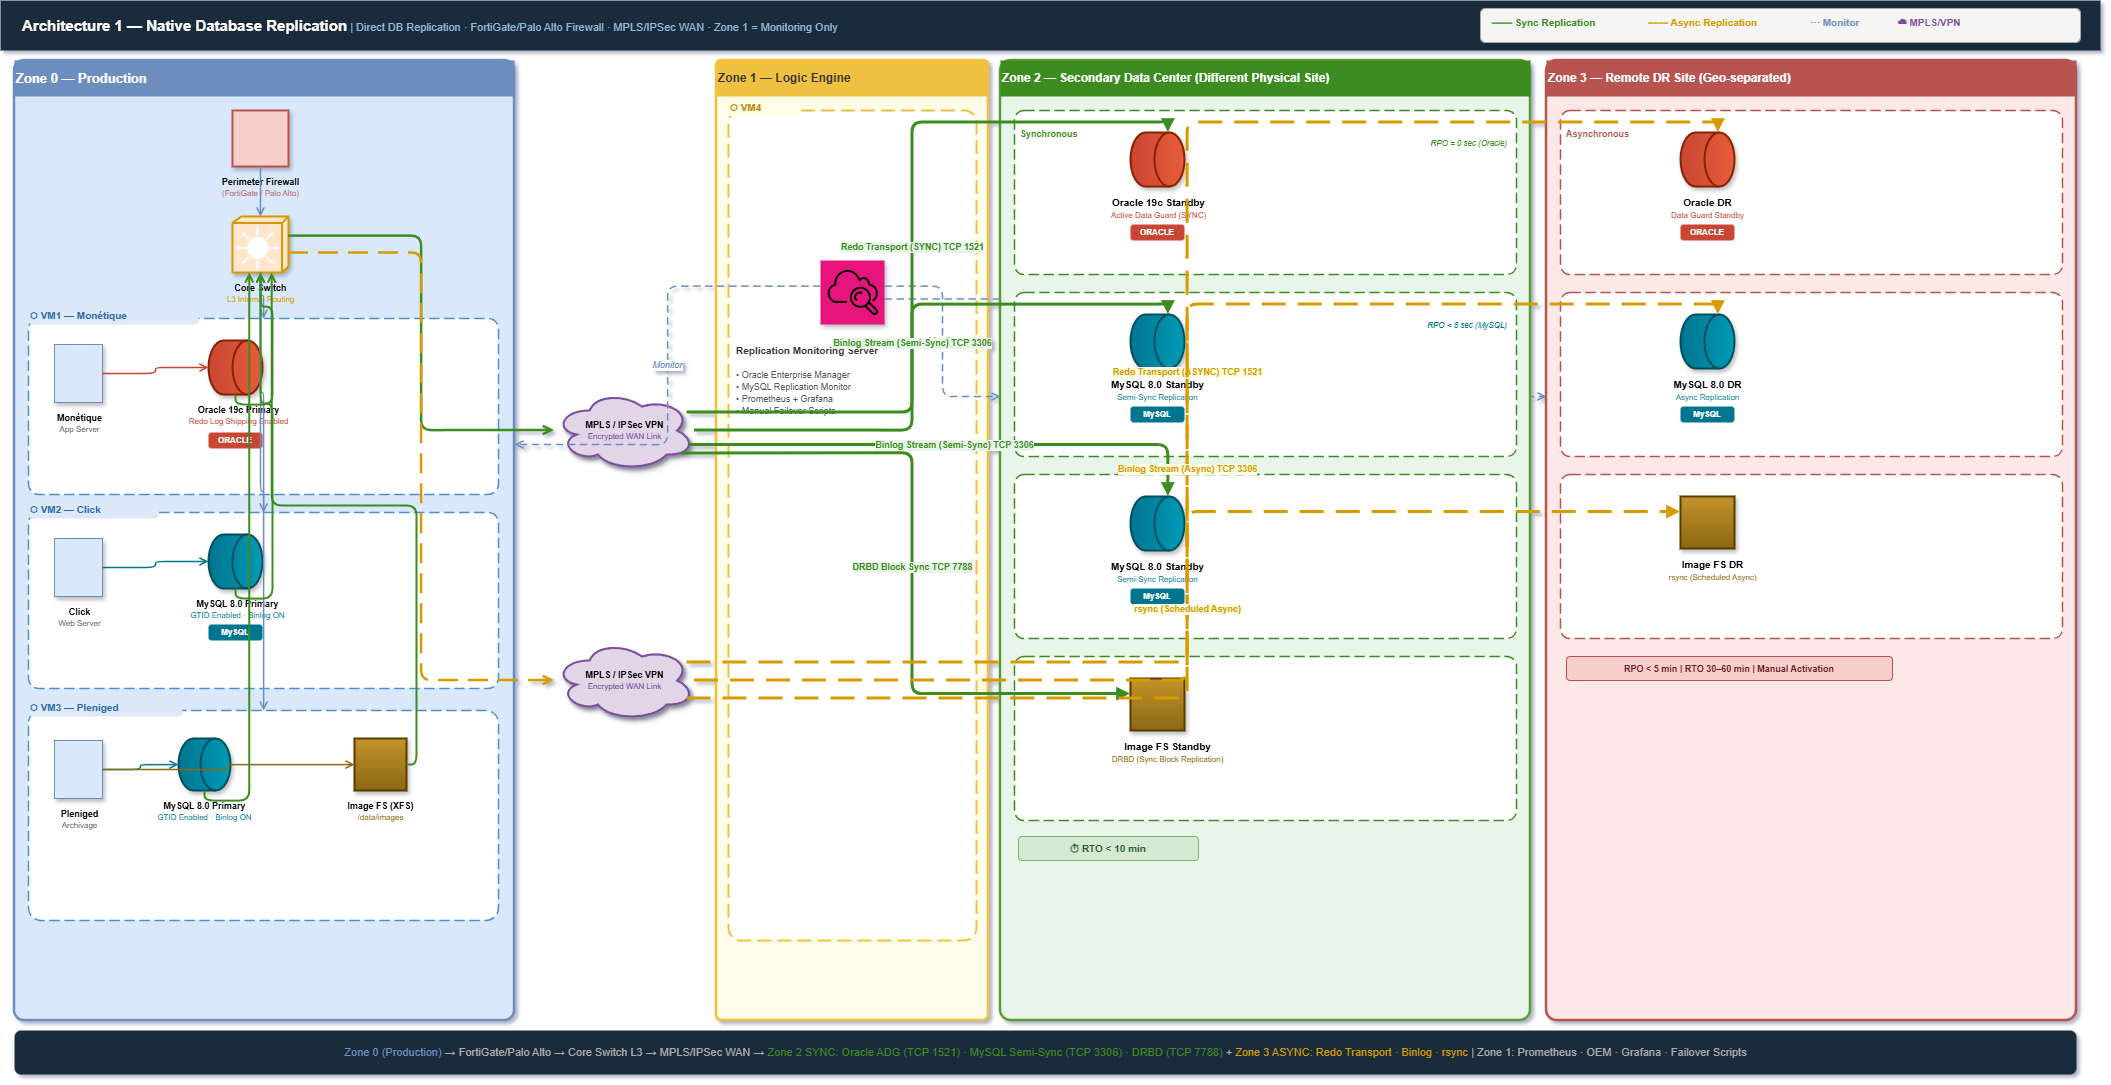
\includegraphics[width=481.878pt,height=247.6729pt]{latexImage_f849d4e5944aecb3c83fcc92746aac90.png}}
\put(172.13,-376.672){\fontsize{10.9091}{1}\usefont{T1}{cmr}{m}{n}\selectfont\color{color_29791}Figure 1: Arc hi tecture DR — Zone 0 a Zone 3}
\put(41.69301,-404.297){\fontsize{10.9091}{1}\usefont{T1}{cmr}{b}{n}\selectfont\color{color_33132}4.2}
\put(57.61811,-404.297){\fontsize{10.9091}{1}\usefont{T1}{cmr}{b}{n}\selectfont\color{color_33132}}
\put(70.0763,-404.297){\fontsize{10.9091}{1}\usefont{T1}{cmr}{b}{n}\selectfont\color{color_33132}Description des Zones}
\put(73.33401,-421.831){\fontsize{10.9091}{1}\usefont{T1}{cmr}{m}{n}\selectfont\color{color_29791}•}
\put(78.75801,-421.831){\fontsize{10.9091}{1}\usefont{T1}{cmr}{b}{n}\selectfont\color{color_29791}}
\put(84.21256,-421.831){\fontsize{10.9091}{1}\usefont{T1}{cmr}{b}{n}\selectfont\color{color_29791}Zone}
\put(210.5007,-421.831){\fontsize{10.9091}{1}\usefont{T1}{cmr}{m}{n}\selectfont\color{color_29791}}
\put(215.3225,-421.831){\fontsize{10.9091}{1}\usefont{T1}{cmr}{m}{n}\selectfont\color{color_29791}Serv eurs primaires protégés par F ortiGate/P alo Alto}
\put(73.33401,-441.856){\fontsize{10.9091}{1}\usefont{T1}{cmr}{m}{n}\selectfont\color{color_29791}•}
\put(78.75801,-441.856){\fontsize{10.9091}{1}\usefont{T1}{cmr}{b}{n}\selectfont\color{color_29791}}
\put(84.21256,-441.856){\fontsize{10.9091}{1}\usefont{T1}{cmr}{b}{n}\selectfont\color{color_29791}Zone}
\put(210.6981,-441.856){\fontsize{10.9091}{1}\usefont{T1}{cmr}{m}{n}\selectfont\color{color_29791}}
\put(215.52,-441.856){\fontsize{10.9091}{1}\usefont{T1}{cmr}{m}{n}\selectfont\color{color_29791}Pro metheus, Grafana, alertes — observ ab ilité uniquemen t}
\put(73.33401,-461.881){\fontsize{10.9091}{1}\usefont{T1}{cmr}{m}{n}\selectfont\color{color_29791}•}
\put(78.75801,-461.881){\fontsize{10.9091}{1}\usefont{T1}{cmr}{b}{n}\selectfont\color{color_29791}}
\put(84.21256,-461.881){\fontsize{10.9091}{1}\usefont{T1}{cmr}{b}{n}\selectfont\color{color_29791}Zone}
\put(280.8502,-461.881){\fontsize{10.9091}{1}\usefont{T1}{cmr}{m}{n}\selectfont\color{color_29791}}
\put(285.672,-461.881){\fontsize{10.9091}{1}\usefont{T1}{cmr}{m}{n}\selectfont\color{color_29791}Réplicas sync/semi-sync, R TO inferieur a 2h}
\put(73.33401,-481.906){\fontsize{10.9091}{1}\usefont{T1}{cmr}{m}{n}\selectfont\color{color_29791}•}
\put(78.75801,-481.906){\fontsize{10.9091}{1}\usefont{T1}{cmr}{b}{n}\selectfont\color{color_29791}}
\put(84.21256,-481.906){\fontsize{10.9091}{1}\usefont{T1}{cmr}{b}{n}\selectfont\color{color_29791}Zone}
\put(278.8407,-481.906){\fontsize{10.9091}{1}\usefont{T1}{cmr}{m}{it}\selectfont\color{color_178741}}
\put(283.5316,-481.906){\fontsize{10.9091}{1}\usefont{T1}{cmr}{m}{it}\selectfont\color{color_178741}[A c onfirmer — in sc op e ou out of sc op e Avril 2026}
\put(84.21301,-495.455){\fontsize{10.9091}{1}\usefont{T1}{cmr}{m}{it}\selectfont\color{color_178741}?]}
\put(41.693,-520.959){\fontsize{10.9091}{1}\usefont{T1}{cmr}{b}{n}\selectfont\color{color_33132}4.3}
\put(57.61811,-520.959){\fontsize{10.9091}{1}\usefont{T1}{cmr}{b}{n}\selectfont\color{color_33132}}
\put(70.0763,-520.959){\fontsize{10.9091}{1}\usefont{T1}{cmr}{b}{n}\selectfont\color{color_33132}Stac k T ec hnologique}
\end{picture}
\begin{tikzpicture}[overlay]
\path(0pt,0pt);
\draw[color_29791,line width=0.398pt]
(41.693pt, -542.16pt) -- (523.583pt, -542.16pt)
;
\draw[color_29791,line width=0.398pt]
(41.892pt, -555.908pt) -- (41.892pt, -542.359pt)
;
\filldraw[color_31474][nonzero rule]
(42.091pt, -555.908pt) -- (123.519pt, -555.908pt)
 -- (123.519pt, -555.908pt)
 -- (123.519pt, -542.359pt)
 -- (123.519pt, -542.359pt)
 -- (42.091pt, -542.359pt) -- cycle
;
\end{tikzpicture}
\begin{picture}(-5,0)(2.5,0)
\put(48.069,-551.843){\fontsize{10.9091}{1}\usefont{T1}{cmr}{b}{n}\selectfont\color{color_283006}Système}
\end{picture}
\begin{tikzpicture}[overlay]
\path(0pt,0pt);
\draw[color_29791,line width=0.398pt]
(123.719pt, -555.908pt) -- (123.719pt, -542.359pt)
;
\filldraw[color_31474][nonzero rule]
(123.918pt, -555.908pt) -- (261.442pt, -555.908pt)
 -- (261.442pt, -555.908pt)
 -- (261.442pt, -542.359pt)
 -- (261.442pt, -542.359pt)
 -- (123.918pt, -542.359pt) -- cycle
;
\end{tikzpicture}
\begin{picture}(-5,0)(2.5,0)
\put(129.896,-551.843){\fontsize{10.9091}{1}\usefont{T1}{cmr}{b}{n}\selectfont\color{color_283006}Réplication}
\end{picture}
\begin{tikzpicture}[overlay]
\path(0pt,0pt);
\draw[color_29791,line width=0.398pt]
(261.642pt, -555.908pt) -- (261.642pt, -542.359pt)
;
\filldraw[color_31474][nonzero rule]
(261.841pt, -555.908pt) -- (458.627pt, -555.908pt)
 -- (458.627pt, -555.908pt)
 -- (458.627pt, -542.359pt)
 -- (458.627pt, -542.359pt)
 -- (261.841pt, -542.359pt) -- cycle
;
\end{tikzpicture}
\begin{picture}(-5,0)(2.5,0)
\put(267.819,-551.843){\fontsize{10.9091}{1}\usefont{T1}{cmr}{b}{n}\selectfont\color{color_283006}Bac kup}
\end{picture}
\begin{tikzpicture}[overlay]
\path(0pt,0pt);
\draw[color_29791,line width=0.398pt]
(458.827pt, -555.908pt) -- (458.827pt, -542.359pt)
;
\filldraw[color_31474][nonzero rule]
(459.026pt, -555.908pt) -- (523.184pt, -555.908pt)
 -- (523.184pt, -555.908pt)
 -- (523.184pt, -542.359pt)
 -- (523.184pt, -542.359pt)
 -- (459.026pt, -542.359pt) -- cycle
;
\end{tikzpicture}
\begin{picture}(-5,0)(2.5,0)
\put(465.004,-551.843){\fontsize{10.9091}{1}\usefont{T1}{cmr}{b}{n}\selectfont\color{color_283006}Proto cole}
\end{picture}
\begin{tikzpicture}[overlay]
\path(0pt,0pt);
\draw[color_29791,line width=0.398pt]
(523.383pt, -555.908pt) -- (523.383pt, -542.359pt)
;
\draw[color_29791,line width=0.398pt]
(41.693pt, -556.107pt) -- (523.583pt, -556.107pt)
;
\draw[color_29791,line width=0.398pt]
(41.892pt, -569.856pt) -- (41.892pt, -556.307pt)
;
\end{tikzpicture}
\begin{picture}(-5,0)(2.5,0)
\put(48.069,-565.791){\fontsize{10.9091}{1}\usefont{T1}{cmr}{b}{n}\selectfont\color{color_29791}Monétique}
\end{picture}
\begin{tikzpicture}[overlay]
\path(0pt,0pt);
\draw[color_29791,line width=0.398pt]
(123.719pt, -569.856pt) -- (123.719pt, -556.307pt)
;
\end{tikzpicture}
\begin{picture}(-5,0)(2.5,0)
\put(129.896,-565.791){\fontsize{10.9091}{1}\usefont{T1}{cmr}{m}{n}\selectfont\color{color_29791}A ctiv e Data Guard (Sync)}
\end{picture}
\begin{tikzpicture}[overlay]
\path(0pt,0pt);
\draw[color_29791,line width=0.398pt]
(261.642pt, -569.856pt) -- (261.642pt, -556.307pt)
;
\end{tikzpicture}
\begin{picture}(-5,0)(2.5,0)
\put(267.819,-565.791){\fontsize{10.9091}{1}\usefont{T1}{cmr}{m}{n}\selectfont\color{color_29791}RMAN + Arc hiv ed Logs}
\end{picture}
\begin{tikzpicture}[overlay]
\path(0pt,0pt);
\draw[color_29791,line width=0.398pt]
(458.827pt, -569.856pt) -- (458.827pt, -556.307pt)
;
\end{tikzpicture}
\begin{picture}(-5,0)(2.5,0)
\put(465.004,-565.791){\fontsize{10.9091}{1}\usefont{T1}{cmr}{m}{n}\selectfont\color{color_29791}TCP 1521}
\end{picture}
\begin{tikzpicture}[overlay]
\path(0pt,0pt);
\draw[color_29791,line width=0.398pt]
(523.383pt, -569.856pt) -- (523.383pt, -556.307pt)
;
\draw[color_29791,line width=0.398pt]
(41.693pt, -570.055pt) -- (523.583pt, -570.055pt)
;
\draw[color_29791,line width=0.398pt]
(41.892pt, -583.803pt) -- (41.892pt, -570.254pt)
;
\filldraw[color_273076][nonzero rule]
(42.091pt, -583.803pt) -- (123.519pt, -583.803pt)
 -- (123.519pt, -583.803pt)
 -- (123.519pt, -570.254pt)
 -- (123.519pt, -570.254pt)
 -- (42.091pt, -570.254pt) -- cycle
;
\end{tikzpicture}
\begin{picture}(-5,0)(2.5,0)
\put(48.069,-579.739){\fontsize{10.9091}{1}\usefont{T1}{cmr}{b}{n}\selectfont\color{color_29791}Clic k}
\end{picture}
\begin{tikzpicture}[overlay]
\path(0pt,0pt);
\draw[color_29791,line width=0.398pt]
(123.719pt, -583.803pt) -- (123.719pt, -570.254pt)
;
\filldraw[color_273076][nonzero rule]
(123.918pt, -583.803pt) -- (261.442pt, -583.803pt)
 -- (261.442pt, -583.803pt)
 -- (261.442pt, -570.254pt)
 -- (261.442pt, -570.254pt)
 -- (123.918pt, -570.254pt) -- cycle
;
\end{tikzpicture}
\begin{picture}(-5,0)(2.5,0)
\put(129.896,-579.739){\fontsize{10.9091}{1}\usefont{T1}{cmr}{m}{n}\selectfont\color{color_29791}MySQL Semi-Sync}
\end{picture}
\begin{tikzpicture}[overlay]
\path(0pt,0pt);
\draw[color_29791,line width=0.398pt]
(261.642pt, -583.803pt) -- (261.642pt, -570.254pt)
;
\filldraw[color_273076][nonzero rule]
(261.841pt, -583.803pt) -- (458.627pt, -583.803pt)
 -- (458.627pt, -583.803pt)
 -- (458.627pt, -570.254pt)
 -- (458.627pt, -570.254pt)
 -- (261.841pt, -570.254pt) -- cycle
;
\end{tikzpicture}
\begin{picture}(-5,0)(2.5,0)
\put(267.819,-579.739){\fontsize{10.9091}{1}\usefont{T1}{cmr}{m}{n}\selectfont\color{color_29791}P ercona XtraBac kup + BinLogs}
\end{picture}
\begin{tikzpicture}[overlay]
\path(0pt,0pt);
\draw[color_29791,line width=0.398pt]
(458.827pt, -583.803pt) -- (458.827pt, -570.254pt)
;
\filldraw[color_273076][nonzero rule]
(459.026pt, -583.803pt) -- (523.184pt, -583.803pt)
 -- (523.184pt, -583.803pt)
 -- (523.184pt, -570.254pt)
 -- (523.184pt, -570.254pt)
 -- (459.026pt, -570.254pt) -- cycle
;
\end{tikzpicture}
\begin{picture}(-5,0)(2.5,0)
\put(465.004,-579.739){\fontsize{10.9091}{1}\usefont{T1}{cmr}{m}{n}\selectfont\color{color_29791}TCP 3306}
\end{picture}
\begin{tikzpicture}[overlay]
\path(0pt,0pt);
\draw[color_29791,line width=0.398pt]
(523.383pt, -583.803pt) -- (523.383pt, -570.254pt)
;
\draw[color_29791,line width=0.398pt]
(41.693pt, -584.003pt) -- (523.583pt, -584.003pt)
;
\draw[color_29791,line width=0.398pt]
(41.892pt, -597.751pt) -- (41.892pt, -584.202pt)
;
\end{tikzpicture}
\begin{picture}(-5,0)(2.5,0)
\put(48.069,-593.686){\fontsize{10.9091}{1}\usefont{T1}{cmr}{b}{n}\selectfont\color{color_29791}Pleniged DB}
\end{picture}
\begin{tikzpicture}[overlay]
\path(0pt,0pt);
\draw[color_29791,line width=0.398pt]
(123.719pt, -597.751pt) -- (123.719pt, -584.202pt)
;
\end{tikzpicture}
\begin{picture}(-5,0)(2.5,0)
\put(129.896,-593.686){\fontsize{10.9091}{1}\usefont{T1}{cmr}{m}{n}\selectfont\color{color_29791}MySQL Semi-Sync}
\end{picture}
\begin{tikzpicture}[overlay]
\path(0pt,0pt);
\draw[color_29791,line width=0.398pt]
(261.642pt, -597.751pt) -- (261.642pt, -584.202pt)
;
\end{tikzpicture}
\begin{picture}(-5,0)(2.5,0)
\put(267.819,-593.686){\fontsize{10.9091}{1}\usefont{T1}{cmr}{m}{n}\selectfont\color{color_29791}P ercona XtraBac kup + BinLogs}
\end{picture}
\begin{tikzpicture}[overlay]
\path(0pt,0pt);
\draw[color_29791,line width=0.398pt]
(458.827pt, -597.751pt) -- (458.827pt, -584.202pt)
;
\end{tikzpicture}
\begin{picture}(-5,0)(2.5,0)
\put(465.004,-593.686){\fontsize{10.9091}{1}\usefont{T1}{cmr}{m}{n}\selectfont\color{color_29791}TCP 3306}
\end{picture}
\begin{tikzpicture}[overlay]
\path(0pt,0pt);
\draw[color_29791,line width=0.398pt]
(523.383pt, -597.751pt) -- (523.383pt, -584.202pt)
;
\draw[color_29791,line width=0.398pt]
(41.693pt, -597.95pt) -- (523.583pt, -597.95pt)
;
\draw[color_29791,line width=0.398pt]
(41.892pt, -611.699pt) -- (41.892pt, -598.15pt)
;
\filldraw[color_273076][nonzero rule]
(42.091pt, -611.699pt) -- (123.519pt, -611.699pt)
 -- (123.519pt, -611.699pt)
 -- (123.519pt, -598.15pt)
 -- (123.519pt, -598.15pt)
 -- (42.091pt, -598.15pt) -- cycle
;
\end{tikzpicture}
\begin{picture}(-5,0)(2.5,0)
\put(48.069,-607.634){\fontsize{10.9091}{1}\usefont{T1}{cmr}{b}{n}\selectfont\color{color_29791}Pleniged FS}
\end{picture}
\begin{tikzpicture}[overlay]
\path(0pt,0pt);
\draw[color_29791,line width=0.398pt]
(123.719pt, -611.699pt) -- (123.719pt, -598.15pt)
;
\filldraw[color_273076][nonzero rule]
(123.918pt, -611.699pt) -- (261.442pt, -611.699pt)
 -- (261.442pt, -611.699pt)
 -- (261.442pt, -598.15pt)
 -- (261.442pt, -598.15pt)
 -- (123.918pt, -598.15pt) -- cycle
;
\end{tikzpicture}
\begin{picture}(-5,0)(2.5,0)
\put(129.896,-607.634){\fontsize{10.9091}{1}\usefont{T1}{cmr}{m}{n}\selectfont\color{color_29791}—}
\end{picture}
\begin{tikzpicture}[overlay]
\path(0pt,0pt);
\draw[color_29791,line width=0.398pt]
(261.642pt, -611.699pt) -- (261.642pt, -598.15pt)
;
\filldraw[color_273076][nonzero rule]
(261.841pt, -611.699pt) -- (458.627pt, -611.699pt)
 -- (458.627pt, -611.699pt)
 -- (458.627pt, -598.15pt)
 -- (458.627pt, -598.15pt)
 -- (261.841pt, -598.15pt) -- cycle
;
\end{tikzpicture}
\begin{picture}(-5,0)(2.5,0)
\put(267.819,-607.634){\fontsize{10.9091}{1}\usefont{T1}{cmr}{m}{n}\selectfont\color{color_29791}rsync nigh tly}
\end{picture}
\begin{tikzpicture}[overlay]
\path(0pt,0pt);
\draw[color_29791,line width=0.398pt]
(458.827pt, -611.699pt) -- (458.827pt, -598.15pt)
;
\filldraw[color_273076][nonzero rule]
(459.026pt, -611.699pt) -- (523.184pt, -611.699pt)
 -- (523.184pt, -611.699pt)
 -- (523.184pt, -598.15pt)
 -- (523.184pt, -598.15pt)
 -- (459.026pt, -598.15pt) -- cycle
;
\end{tikzpicture}
\begin{picture}(-5,0)(2.5,0)
\put(465.004,-607.634){\fontsize{10.9091}{1}\usefont{T1}{cmr}{m}{n}\selectfont\color{color_29791}SSH}
\end{picture}
\begin{tikzpicture}[overlay]
\path(0pt,0pt);
\draw[color_29791,line width=0.398pt]
(523.383pt, -611.699pt) -- (523.383pt, -598.15pt)
;
\draw[color_29791,line width=0.398pt]
(41.693pt, -611.898pt) -- (523.583pt, -611.898pt)
;
\end{tikzpicture}
\begin{picture}(-5,0)(2.5,0)
\put(70.328,-636.605){\fontsize{10.9091}{1}\usefont{T1}{cmr}{m}{n}\selectfont\color{color_29791}T able 4: Stac k DR par système — Monitoring : OEM + Prometheus + Grafana sur tous}
\put(41.693,-664.629){\fontsize{11.9552}{1}\usefont{T1}{cmr}{b}{n}\selectfont\color{color_31474}5}
\put(48.41661,-664.629){\fontsize{11.9552}{1}\usefont{T1}{cmr}{b}{n}\selectfont\color{color_31474}}
\put(61.86621,-664.629){\fontsize{11.9552}{1}\usefont{T1}{cmr}{b}{n}\selectfont\color{color_31474}Ob jectifs R TO / RPO}
\end{picture}
\begin{tikzpicture}[overlay]
\path(0pt,0pt);
\draw[color_31474,line width=0.797pt]
(41.693pt, -671.204pt) -- (523.583pt, -671.204pt)
;
\draw[color_29791,line width=0.398pt]
(41.693pt, -777.389pt) -- (523.583pt, -777.389pt)
;
\end{tikzpicture}
\begin{picture}(-5,0)(2.5,0)
\put(271.848,-790.022){\fontsize{9.9626}{1}\usefont{T1}{cmr}{m}{n}\selectfont\color{color_109231}4}
\put(293.424,-790.022){\fontsize{9.9626}{1}\usefont{T1}{cmr}{m}{n}\selectfont\color{color_109231}}
\put(407.2965,-790.022){\fontsize{9.9626}{1}\usefont{T1}{cmr}{m}{n}\selectfont\color{color_109231}Usage In terne Uniquemen t}
\end{picture}
\newpage
\begin{tikzpicture}[overlay]\path(0pt,0pt);\end{tikzpicture}
\begin{picture}(-5,0)(2.5,0)
\put(41.693,-31.48297){\fontsize{9.9626}{1}\usefont{T1}{cmr}{b}{n}\selectfont\color{color_31474}BNM}
\put(150.0482,-31.48297){\fontsize{9.9626}{1}\usefont{T1}{cmr}{m}{n}\selectfont\color{color_109231}}
\put(348.1446,-31.48297){\fontsize{9.9626}{1}\usefont{T1}{cmr}{m}{n}\selectfont\color{color_109231}Blueprin t DR v1.0 — CONFIDENTIEL}
\end{picture}
\begin{tikzpicture}[overlay]
\path(0pt,0pt);
\draw[color_29791,line width=0.398pt]
(41.693pt, -35.26898pt) -- (523.583pt, -35.26898pt)
;
\draw[color_29791,line width=0.398pt]
(41.693pt, -60.17603pt) -- (523.583pt, -60.17603pt)
;
\draw[color_29791,line width=0.398pt]
(41.892pt, -73.92401pt) -- (41.892pt, -60.375pt)
;
\filldraw[color_31474][nonzero rule]
(42.091pt, -73.92401pt) -- (123.519pt, -73.92401pt)
 -- (123.519pt, -73.92401pt)
 -- (123.519pt, -60.375pt)
 -- (123.519pt, -60.375pt)
 -- (42.091pt, -60.375pt) -- cycle
;
\end{tikzpicture}
\begin{picture}(-5,0)(2.5,0)
\put(48.069,-69.85901){\fontsize{10.9091}{1}\usefont{T1}{cmr}{b}{n}\selectfont\color{color_283006}Système}
\end{picture}
\begin{tikzpicture}[overlay]
\path(0pt,0pt);
\draw[color_29791,line width=0.398pt]
(123.719pt, -73.92401pt) -- (123.719pt, -60.375pt)
;
\filldraw[color_31474][nonzero rule]
(123.918pt, -73.92401pt) -- (237.842pt, -73.92401pt)
 -- (237.842pt, -73.92401pt)
 -- (237.842pt, -60.375pt)
 -- (237.842pt, -60.375pt)
 -- (123.918pt, -60.375pt) -- cycle
;
\end{tikzpicture}
\begin{picture}(-5,0)(2.5,0)
\put(129.896,-69.85901){\fontsize{10.9091}{1}\usefont{T1}{cmr}{b}{n}\selectfont\color{color_283006}Tier}
\end{picture}
\begin{tikzpicture}[overlay]
\path(0pt,0pt);
\draw[color_29791,line width=0.398pt]
(238.042pt, -73.92401pt) -- (238.042pt, -60.375pt)
;
\filldraw[color_31474][nonzero rule]
(238.241pt, -73.92401pt) -- (277.375pt, -73.92401pt)
 -- (277.375pt, -73.92401pt)
 -- (277.375pt, -60.375pt)
 -- (277.375pt, -60.375pt)
 -- (238.241pt, -60.375pt) -- cycle
;
\end{tikzpicture}
\begin{picture}(-5,0)(2.5,0)
\put(244.218,-69.85901){\fontsize{10.9091}{1}\usefont{T1}{cmr}{b}{n}\selectfont\color{color_283006}RPO}
\end{picture}
\begin{tikzpicture}[overlay]
\path(0pt,0pt);
\draw[color_29791,line width=0.398pt]
(277.575pt, -73.92401pt) -- (277.575pt, -60.375pt)
;
\filldraw[color_31474][nonzero rule]
(277.774pt, -73.92401pt) -- (316.026pt, -73.92401pt)
 -- (316.026pt, -73.92401pt)
 -- (316.026pt, -60.375pt)
 -- (316.026pt, -60.375pt)
 -- (277.774pt, -60.375pt) -- cycle
;
\end{tikzpicture}
\begin{picture}(-5,0)(2.5,0)
\put(283.751,-69.85901){\fontsize{10.9091}{1}\usefont{T1}{cmr}{b}{n}\selectfont\color{color_283006}R TO}
\end{picture}
\begin{tikzpicture}[overlay]
\path(0pt,0pt);
\draw[color_29791,line width=0.398pt]
(316.225pt, -73.92401pt) -- (316.225pt, -60.375pt)
;
\filldraw[color_31474][nonzero rule]
(316.424pt, -73.92401pt) -- (523.184pt, -73.92401pt)
 -- (523.184pt, -73.92401pt)
 -- (523.184pt, -60.375pt)
 -- (523.184pt, -60.375pt)
 -- (316.424pt, -60.375pt) -- cycle
;
\end{tikzpicture}
\begin{picture}(-5,0)(2.5,0)
\put(322.402,-69.85901){\fontsize{10.9091}{1}\usefont{T1}{cmr}{b}{n}\selectfont\color{color_283006}Garan tie}
\end{picture}
\begin{tikzpicture}[overlay]
\path(0pt,0pt);
\draw[color_29791,line width=0.398pt]
(523.383pt, -73.92401pt) -- (523.383pt, -60.375pt)
;
\draw[color_29791,line width=0.398pt]
(41.693pt, -74.12299pt) -- (523.583pt, -74.12299pt)
;
\draw[color_29791,line width=0.398pt]
(41.892pt, -87.87201pt) -- (41.892pt, -74.323pt)
;
\end{tikzpicture}
\begin{picture}(-5,0)(2.5,0)
\put(48.069,-83.80701){\fontsize{10.9091}{1}\usefont{T1}{cmr}{b}{n}\selectfont\color{color_29791}Monétique}
\end{picture}
\begin{tikzpicture}[overlay]
\path(0pt,0pt);
\draw[color_29791,line width=0.398pt]
(123.719pt, -87.87201pt) -- (123.719pt, -74.323pt)
;
\end{tikzpicture}
\begin{picture}(-5,0)(2.5,0)
\put(129.896,-83.80701){\fontsize{10.9091}{1}\usefont{T1}{cmr}{m}{n}\selectfont\color{color_29791}1 — Mission Critique}
\end{picture}
\begin{tikzpicture}[overlay]
\path(0pt,0pt);
\draw[color_29791,line width=0.398pt]
(238.042pt, -87.87201pt) -- (238.042pt, -74.323pt)
;
\end{tikzpicture}
\begin{picture}(-5,0)(2.5,0)
\put(244.218,-83.80701){\fontsize{10.9091}{1}\usefont{T1}{cmr}{b}{n}\selectfont\color{color_33759}0}
\end{picture}
\begin{tikzpicture}[overlay]
\path(0pt,0pt);
\draw[color_29791,line width=0.398pt]
(277.575pt, -87.87201pt) -- (277.575pt, -74.323pt)
;
\end{tikzpicture}
\begin{picture}(-5,0)(2.5,0)
\put(283.751,-83.80701){\fontsize{10.9091}{1}\usefont{T1}{cmr}{m}{n}\selectfont\color{color_29791}1–2 h}
\end{picture}
\begin{tikzpicture}[overlay]
\path(0pt,0pt);
\draw[color_29791,line width=0.398pt]
(316.225pt, -87.87201pt) -- (316.225pt, -74.323pt)
;
\end{tikzpicture}
\begin{picture}(-5,0)(2.5,0)
\put(322.402,-83.80701){\fontsize{10.9091}{1}\usefont{T1}{cmr}{m}{n}\selectfont\color{color_29791}Data Guard sync hrone}
\end{picture}
\begin{tikzpicture}[overlay]
\path(0pt,0pt);
\draw[color_29791,line width=0.398pt]
(523.383pt, -87.87201pt) -- (523.383pt, -74.323pt)
;
\draw[color_29791,line width=0.398pt]
(41.693pt, -88.07098pt) -- (523.583pt, -88.07098pt)
;
\draw[color_29791,line width=0.398pt]
(41.892pt, -101.819pt) -- (41.892pt, -88.26996pt)
;
\filldraw[color_273076][nonzero rule]
(42.091pt, -101.819pt) -- (123.519pt, -101.819pt)
 -- (123.519pt, -101.819pt)
 -- (123.519pt, -88.26996pt)
 -- (123.519pt, -88.26996pt)
 -- (42.091pt, -88.26996pt) -- cycle
;
\end{tikzpicture}
\begin{picture}(-5,0)(2.5,0)
\put(48.069,-97.755){\fontsize{10.9091}{1}\usefont{T1}{cmr}{b}{n}\selectfont\color{color_29791}Clic k}
\end{picture}
\begin{tikzpicture}[overlay]
\path(0pt,0pt);
\draw[color_29791,line width=0.398pt]
(123.719pt, -101.819pt) -- (123.719pt, -88.26996pt)
;
\filldraw[color_273076][nonzero rule]
(123.918pt, -101.819pt) -- (237.842pt, -101.819pt)
 -- (237.842pt, -101.819pt)
 -- (237.842pt, -88.26996pt)
 -- (237.842pt, -88.26996pt)
 -- (123.918pt, -88.26996pt) -- cycle
;
\end{tikzpicture}
\begin{picture}(-5,0)(2.5,0)
\put(129.896,-97.755){\fontsize{10.9091}{1}\usefont{T1}{cmr}{m}{n}\selectfont\color{color_29791}2 — Critique}
\end{picture}
\begin{tikzpicture}[overlay]
\path(0pt,0pt);
\draw[color_29791,line width=0.398pt]
(238.042pt, -101.819pt) -- (238.042pt, -88.26996pt)
;
\filldraw[color_273076][nonzero rule]
(238.241pt, -101.819pt) -- (277.375pt, -101.819pt)
 -- (277.375pt, -101.819pt)
 -- (277.375pt, -88.26996pt)
 -- (277.375pt, -88.26996pt)
 -- (238.241pt, -88.26996pt) -- cycle
;
\end{tikzpicture}
\begin{picture}(-5,0)(2.5,0)
\put(244.218,-97.755){\fontsize{10.9091}{1}\usefont{T1}{cmr}{m}{it}\selectfont\color{color_33759}∼ 0}
\end{picture}
\begin{tikzpicture}[overlay]
\path(0pt,0pt);
\draw[color_29791,line width=0.398pt]
(277.575pt, -101.819pt) -- (277.575pt, -88.26996pt)
;
\filldraw[color_273076][nonzero rule]
(277.774pt, -101.819pt) -- (316.026pt, -101.819pt)
 -- (316.026pt, -101.819pt)
 -- (316.026pt, -88.26996pt)
 -- (316.026pt, -88.26996pt)
 -- (277.774pt, -88.26996pt) -- cycle
;
\end{tikzpicture}
\begin{picture}(-5,0)(2.5,0)
\put(283.751,-97.755){\fontsize{10.9091}{1}\usefont{T1}{cmr}{m}{n}\selectfont\color{color_29791}2–4 h}
\end{picture}
\begin{tikzpicture}[overlay]
\path(0pt,0pt);
\draw[color_29791,line width=0.398pt]
(316.225pt, -101.819pt) -- (316.225pt, -88.26996pt)
;
\filldraw[color_273076][nonzero rule]
(316.424pt, -101.819pt) -- (523.184pt, -101.819pt)
 -- (523.184pt, -101.819pt)
 -- (523.184pt, -88.26996pt)
 -- (523.184pt, -88.26996pt)
 -- (316.424pt, -88.26996pt) -- cycle
;
\end{tikzpicture}
\begin{picture}(-5,0)(2.5,0)
\put(322.402,-97.755){\fontsize{10.9091}{1}\usefont{T1}{cmr}{m}{n}\selectfont\color{color_29791}MySQL semi-sync}
\end{picture}
\begin{tikzpicture}[overlay]
\path(0pt,0pt);
\draw[color_29791,line width=0.398pt]
(523.383pt, -101.819pt) -- (523.383pt, -88.26996pt)
;
\draw[color_29791,line width=0.398pt]
(41.693pt, -102.019pt) -- (523.583pt, -102.019pt)
;
\draw[color_29791,line width=0.398pt]
(41.892pt, -115.767pt) -- (41.892pt, -102.218pt)
;
\end{tikzpicture}
\begin{picture}(-5,0)(2.5,0)
\put(48.069,-111.702){\fontsize{10.9091}{1}\usefont{T1}{cmr}{b}{n}\selectfont\color{color_29791}Pleniged DB}
\end{picture}
\begin{tikzpicture}[overlay]
\path(0pt,0pt);
\draw[color_29791,line width=0.398pt]
(123.719pt, -115.767pt) -- (123.719pt, -102.218pt)
;
\end{tikzpicture}
\begin{picture}(-5,0)(2.5,0)
\put(129.896,-111.702){\fontsize{10.9091}{1}\usefont{T1}{cmr}{m}{n}\selectfont\color{color_29791}2 — Critique}
\end{picture}
\begin{tikzpicture}[overlay]
\path(0pt,0pt);
\draw[color_29791,line width=0.398pt]
(238.042pt, -115.767pt) -- (238.042pt, -102.218pt)
;
\end{tikzpicture}
\begin{picture}(-5,0)(2.5,0)
\put(244.218,-111.702){\fontsize{10.9091}{1}\usefont{T1}{cmr}{m}{it}\selectfont\color{color_33759}∼ 0}
\end{picture}
\begin{tikzpicture}[overlay]
\path(0pt,0pt);
\draw[color_29791,line width=0.398pt]
(277.575pt, -115.767pt) -- (277.575pt, -102.218pt)
;
\end{tikzpicture}
\begin{picture}(-5,0)(2.5,0)
\put(283.751,-111.702){\fontsize{10.9091}{1}\usefont{T1}{cmr}{m}{n}\selectfont\color{color_29791}2–4 h}
\end{picture}
\begin{tikzpicture}[overlay]
\path(0pt,0pt);
\draw[color_29791,line width=0.398pt]
(316.225pt, -115.767pt) -- (316.225pt, -102.218pt)
;
\end{tikzpicture}
\begin{picture}(-5,0)(2.5,0)
\put(322.402,-111.702){\fontsize{10.9091}{1}\usefont{T1}{cmr}{m}{n}\selectfont\color{color_29791}MySQL semi-sync}
\end{picture}
\begin{tikzpicture}[overlay]
\path(0pt,0pt);
\draw[color_29791,line width=0.398pt]
(523.383pt, -115.767pt) -- (523.383pt, -102.218pt)
;
\draw[color_29791,line width=0.398pt]
(41.693pt, -115.966pt) -- (523.583pt, -115.966pt)
;
\draw[color_29791,line width=0.398pt]
(41.892pt, -129.715pt) -- (41.892pt, -116.166pt)
;
\filldraw[color_273076][nonzero rule]
(42.091pt, -129.715pt) -- (123.519pt, -129.715pt)
 -- (123.519pt, -129.715pt)
 -- (123.519pt, -116.166pt)
 -- (123.519pt, -116.166pt)
 -- (42.091pt, -116.166pt) -- cycle
;
\end{tikzpicture}
\begin{picture}(-5,0)(2.5,0)
\put(48.069,-125.65){\fontsize{10.9091}{1}\usefont{T1}{cmr}{b}{n}\selectfont\color{color_29791}Pleniged FS}
\end{picture}
\begin{tikzpicture}[overlay]
\path(0pt,0pt);
\draw[color_29791,line width=0.398pt]
(123.719pt, -129.715pt) -- (123.719pt, -116.166pt)
;
\filldraw[color_273076][nonzero rule]
(123.918pt, -129.715pt) -- (237.842pt, -129.715pt)
 -- (237.842pt, -129.715pt)
 -- (237.842pt, -116.166pt)
 -- (237.842pt, -116.166pt)
 -- (123.918pt, -116.166pt) -- cycle
;
\end{tikzpicture}
\begin{picture}(-5,0)(2.5,0)
\put(129.896,-125.65){\fontsize{10.9091}{1}\usefont{T1}{cmr}{m}{n}\selectfont\color{color_29791}3 — Imp orta n t}
\end{picture}
\begin{tikzpicture}[overlay]
\path(0pt,0pt);
\draw[color_29791,line width=0.398pt]
(238.042pt, -129.715pt) -- (238.042pt, -116.166pt)
;
\filldraw[color_273076][nonzero rule]
(238.241pt, -129.715pt) -- (277.375pt, -129.715pt)
 -- (277.375pt, -129.715pt)
 -- (277.375pt, -116.166pt)
 -- (277.375pt, -116.166pt)
 -- (238.241pt, -116.166pt) -- cycle
;
\end{tikzpicture}
\begin{picture}(-5,0)(2.5,0)
\put(244.218,-125.65){\fontsize{10.9091}{1}\usefont{T1}{cmr}{m}{n}\selectfont\color{color_29791}24 h}
\end{picture}
\begin{tikzpicture}[overlay]
\path(0pt,0pt);
\draw[color_29791,line width=0.398pt]
(277.575pt, -129.715pt) -- (277.575pt, -116.166pt)
;
\filldraw[color_273076][nonzero rule]
(277.774pt, -129.715pt) -- (316.026pt, -129.715pt)
 -- (316.026pt, -129.715pt)
 -- (316.026pt, -116.166pt)
 -- (316.026pt, -116.166pt)
 -- (277.774pt, -116.166pt) -- cycle
;
\end{tikzpicture}
\begin{picture}(-5,0)(2.5,0)
\put(283.751,-125.65){\fontsize{10.9091}{1}\usefont{T1}{cmr}{m}{n}\selectfont\color{color_29791}24 h}
\end{picture}
\begin{tikzpicture}[overlay]
\path(0pt,0pt);
\draw[color_29791,line width=0.398pt]
(316.225pt, -129.715pt) -- (316.225pt, -116.166pt)
;
\filldraw[color_273076][nonzero rule]
(316.424pt, -129.715pt) -- (523.184pt, -129.715pt)
 -- (523.184pt, -129.715pt)
 -- (523.184pt, -116.166pt)
 -- (523.184pt, -116.166pt)
 -- (316.424pt, -116.166pt) -- cycle
;
\end{tikzpicture}
\begin{picture}(-5,0)(2.5,0)
\put(322.402,-125.65){\fontsize{10.9091}{1}\usefont{T1}{cmr}{m}{n}\selectfont\color{color_29791}rsync nigh tly}
\end{picture}
\begin{tikzpicture}[overlay]
\path(0pt,0pt);
\draw[color_29791,line width=0.398pt]
(523.383pt, -129.715pt) -- (523.383pt, -116.166pt)
;
\draw[color_29791,line width=0.398pt]
(41.693pt, -129.914pt) -- (523.583pt, -129.914pt)
;
\end{tikzpicture}
\begin{picture}(-5,0)(2.5,0)
\put(41.693,-154.621){\fontsize{10.9091}{1}\usefont{T1}{cmr}{m}{n}\selectfont\color{color_29791}T able 5: Ob jectifs R TO/RPO v a lidés — RPO 0 garan ti : aucune tran saction v alidée sa ns confirmation}
\put(41.693,-168.171){\fontsize{10.9091}{1}\usefont{T1}{cmr}{m}{n}\selectfont\color{color_29791}replica}
\put(41.693,-194.298){\fontsize{11.9552}{1}\usefont{T1}{cmr}{b}{n}\selectfont\color{color_31474}6}
\put(48.41661,-194.298){\fontsize{11.9552}{1}\usefont{T1}{cmr}{b}{n}\selectfont\color{color_31474}}
\put(61.86621,-194.298){\fontsize{11.9552}{1}\usefont{T1}{cmr}{b}{n}\selectfont\color{color_31474}Infrastructure — Une VM par Zone}
\end{picture}
\begin{tikzpicture}[overlay]
\path(0pt,0pt);
\draw[color_31474,line width=0.797pt]
(41.693pt, -200.874pt) -- (523.583pt, -200.874pt)
;
\draw[color_29791,line width=0.398pt]
(41.693pt, -221.494pt) -- (523.583pt, -221.494pt)
;
\draw[color_29791,line width=0.398pt]
(41.892pt, -235.242pt) -- (41.892pt, -221.693pt)
;
\filldraw[color_31474][nonzero rule]
(42.091pt, -235.242pt) -- (90.901pt, -235.242pt)
 -- (90.901pt, -235.242pt)
 -- (90.901pt, -221.693pt)
 -- (90.901pt, -221.693pt)
 -- (42.091pt, -221.693pt) -- cycle
;
\end{tikzpicture}
\begin{picture}(-5,0)(2.5,0)
\put(48.069,-231.177){\fontsize{10.9091}{1}\usefont{T1}{cmr}{b}{n}\selectfont\color{color_283006}Zone}
\end{picture}
\begin{tikzpicture}[overlay]
\path(0pt,0pt);
\draw[color_29791,line width=0.398pt]
(91.101pt, -235.242pt) -- (91.101pt, -221.693pt)
;
\filldraw[color_31474][nonzero rule]
(91.3pt, -235.242pt) -- (381.091pt, -235.242pt)
 -- (381.091pt, -235.242pt)
 -- (381.091pt, -221.693pt)
 -- (381.091pt, -221.693pt)
 -- (91.3pt, -221.693pt) -- cycle
;
\end{tikzpicture}
\begin{picture}(-5,0)(2.5,0)
\put(97.277,-231.177){\fontsize{10.9091}{1}\usefont{T1}{cmr}{b}{n}\selectfont\color{color_283006}Rôles}
\end{picture}
\begin{tikzpicture}[overlay]
\path(0pt,0pt);
\draw[color_29791,line width=0.398pt]
(381.29pt, -235.242pt) -- (381.29pt, -221.693pt)
;
\filldraw[color_31474][nonzero rule]
(381.49pt, -235.242pt) -- (423.977pt, -235.242pt)
 -- (423.977pt, -235.242pt)
 -- (423.977pt, -221.693pt)
 -- (423.977pt, -221.693pt)
 -- (381.49pt, -221.693pt) -- cycle
;
\end{tikzpicture}
\begin{picture}(-5,0)(2.5,0)
\put(387.467,-231.177){\fontsize{10.9091}{1}\usefont{T1}{cmr}{b}{n}\selectfont\color{color_283006}RAM}
\end{picture}
\begin{tikzpicture}[overlay]
\path(0pt,0pt);
\draw[color_29791,line width=0.398pt]
(424.176pt, -235.242pt) -- (424.176pt, -221.693pt)
;
\filldraw[color_31474][nonzero rule]
(424.375pt, -235.242pt) -- (463.416pt, -235.242pt)
 -- (463.416pt, -235.242pt)
 -- (463.416pt, -221.693pt)
 -- (463.416pt, -221.693pt)
 -- (424.375pt, -221.693pt) -- cycle
;
\end{tikzpicture}
\begin{picture}(-5,0)(2.5,0)
\put(430.353,-231.177){\fontsize{10.9091}{1}\usefont{T1}{cmr}{b}{n}\selectfont\color{color_283006}CPU}
\end{picture}
\begin{tikzpicture}[overlay]
\path(0pt,0pt);
\draw[color_29791,line width=0.398pt]
(463.616pt, -235.242pt) -- (463.616pt, -221.693pt)
;
\filldraw[color_31474][nonzero rule]
(463.815pt, -235.242pt) -- (523.184pt, -235.242pt)
 -- (523.184pt, -235.242pt)
 -- (523.184pt, -221.693pt)
 -- (523.184pt, -221.693pt)
 -- (463.815pt, -221.693pt) -- cycle
;
\end{tikzpicture}
\begin{picture}(-5,0)(2.5,0)
\put(469.792,-231.177){\fontsize{10.9091}{1}\usefont{T1}{cmr}{b}{n}\selectfont\color{color_283006}Sto c k age}
\end{picture}
\begin{tikzpicture}[overlay]
\path(0pt,0pt);
\draw[color_29791,line width=0.398pt]
(523.383pt, -235.242pt) -- (523.383pt, -221.693pt)
;
\draw[color_29791,line width=0.398pt]
(41.693pt, -235.441pt) -- (523.583pt, -235.441pt)
;
\draw[color_29791,line width=0.398pt]
(41.892pt, -262.739pt) -- (41.892pt, -235.641pt)
;
\end{tikzpicture}
\begin{picture}(-5,0)(2.5,0)
\put(48.069,-245.125){\fontsize{10.9091}{1}\usefont{T1}{cmr}{b}{n}\selectfont\color{color_29791}Zone 1}
\end{picture}
\begin{tikzpicture}[overlay]
\path(0pt,0pt);
\draw[color_29791,line width=0.398pt]
(91.101pt, -262.739pt) -- (91.101pt, -235.641pt)
;
\end{tikzpicture}
\begin{picture}(-5,0)(2.5,0)
\put(97.277,-245.125){\fontsize{10.9091}{1}\usefont{T1}{cmr}{m}{n}\selectfont\color{color_29791}Monitoring — Prometheus, Grafana, Alertmanager, OEM,}
\put(97.277,-258.674){\fontsize{10.9091}{1}\usefont{T1}{cmr}{m}{n}\selectfont\color{color_29791}MySQL Mon itor}
\end{picture}
\begin{tikzpicture}[overlay]
\path(0pt,0pt);
\draw[color_29791,line width=0.398pt]
(381.29pt, -262.739pt) -- (381.29pt, -235.641pt)
;
\end{tikzpicture}
\begin{picture}(-5,0)(2.5,0)
\put(387.467,-245.125){\fontsize{10.9091}{1}\usefont{T1}{cmr}{m}{n}\selectfont\color{color_29791}8 GB}
\end{picture}
\begin{tikzpicture}[overlay]
\path(0pt,0pt);
\draw[color_29791,line width=0.398pt]
(424.176pt, -262.739pt) -- (424.176pt, -235.641pt)
;
\end{tikzpicture}
\begin{picture}(-5,0)(2.5,0)
\put(430.353,-245.125){\fontsize{10.9091}{1}\usefont{T1}{cmr}{m}{n}\selectfont\color{color_29791}4c}
\end{picture}
\begin{tikzpicture}[overlay]
\path(0pt,0pt);
\draw[color_29791,line width=0.398pt]
(463.616pt, -262.739pt) -- (463.616pt, -235.641pt)
;
\end{tikzpicture}
\begin{picture}(-5,0)(2.5,0)
\put(469.792,-245.125){\fontsize{10.9091}{1}\usefont{T1}{cmr}{m}{n}\selectfont\color{color_29791}200 GB}
\end{picture}
\begin{tikzpicture}[overlay]
\path(0pt,0pt);
\draw[color_29791,line width=0.398pt]
(523.383pt, -262.739pt) -- (523.383pt, -235.641pt)
;
\draw[color_29791,line width=0.398pt]
(41.693pt, -262.938pt) -- (523.583pt, -262.938pt)
;
\draw[color_29791,line width=0.398pt]
(41.892pt, -290.236pt) -- (41.892pt, -263.138pt)
;
\filldraw[color_273076][nonzero rule]
(42.091pt, -290.236pt) -- (90.901pt, -290.236pt)
 -- (90.901pt, -290.236pt)
 -- (90.901pt, -263.138pt)
 -- (90.901pt, -263.138pt)
 -- (42.091pt, -263.138pt) -- cycle
;
\end{tikzpicture}
\begin{picture}(-5,0)(2.5,0)
\put(48.069,-272.622){\fontsize{10.9091}{1}\usefont{T1}{cmr}{b}{n}\selectfont\color{color_29791}Zone 2}
\end{picture}
\begin{tikzpicture}[overlay]
\path(0pt,0pt);
\draw[color_29791,line width=0.398pt]
(91.101pt, -290.236pt) -- (91.101pt, -263.138pt)
;
\filldraw[color_273076][nonzero rule]
(91.3pt, -290.236pt) -- (381.091pt, -290.236pt)
 -- (381.091pt, -290.236pt)
 -- (381.091pt, -263.138pt)
 -- (381.091pt, -263.138pt)
 -- (91.3pt, -263.138pt) -- cycle
;
\end{tikzpicture}
\begin{picture}(-5,0)(2.5,0)
\put(97.277,-272.622){\fontsize{10.9091}{1}\usefont{T1}{cmr}{m}{n}\selectfont\color{color_29791}Oracle Logical Standb y + MySQL Replica semi-sync (Clic k}
\put(97.277,-286.171){\fontsize{10.9091}{1}\usefont{T1}{cmr}{m}{n}\selectfont\color{color_29791}+ Plen iged) + rsync FS}
\end{picture}
\begin{tikzpicture}[overlay]
\path(0pt,0pt);
\draw[color_29791,line width=0.398pt]
(381.29pt, -290.236pt) -- (381.29pt, -263.138pt)
;
\filldraw[color_273076][nonzero rule]
(381.49pt, -290.236pt) -- (423.977pt, -290.236pt)
 -- (423.977pt, -290.236pt)
 -- (423.977pt, -263.138pt)
 -- (423.977pt, -263.138pt)
 -- (381.49pt, -263.138pt) -- cycle
;
\end{tikzpicture}
\begin{picture}(-5,0)(2.5,0)
\put(387.467,-272.622){\fontsize{10.9091}{1}\usefont{T1}{cmr}{m}{n}\selectfont\color{color_29791}8 GB}
\end{picture}
\begin{tikzpicture}[overlay]
\path(0pt,0pt);
\draw[color_29791,line width=0.398pt]
(424.176pt, -290.236pt) -- (424.176pt, -263.138pt)
;
\filldraw[color_273076][nonzero rule]
(424.375pt, -290.236pt) -- (463.416pt, -290.236pt)
 -- (463.416pt, -290.236pt)
 -- (463.416pt, -263.138pt)
 -- (463.416pt, -263.138pt)
 -- (424.375pt, -263.138pt) -- cycle
;
\end{tikzpicture}
\begin{picture}(-5,0)(2.5,0)
\put(430.353,-272.622){\fontsize{10.9091}{1}\usefont{T1}{cmr}{m}{n}\selectfont\color{color_29791}20c}
\end{picture}
\begin{tikzpicture}[overlay]
\path(0pt,0pt);
\draw[color_29791,line width=0.398pt]
(463.616pt, -290.236pt) -- (463.616pt, -263.138pt)
;
\filldraw[color_273076][nonzero rule]
(463.815pt, -290.236pt) -- (523.184pt, -290.236pt)
 -- (523.184pt, -290.236pt)
 -- (523.184pt, -263.138pt)
 -- (523.184pt, -263.138pt)
 -- (463.815pt, -263.138pt) -- cycle
;
\end{tikzpicture}
\begin{picture}(-5,0)(2.5,0)
\put(469.792,-272.622){\fontsize{10.9091}{1}\usefont{T1}{cmr}{m}{n}\selectfont\color{color_29791}11.4 TB}
\end{picture}
\begin{tikzpicture}[overlay]
\path(0pt,0pt);
\draw[color_29791,line width=0.398pt]
(523.383pt, -290.236pt) -- (523.383pt, -263.138pt)
;
\draw[color_29791,line width=0.398pt]
(41.693pt, -290.435pt) -- (523.583pt, -290.435pt)
;
\draw[color_29791,line width=0.398pt]
(41.892pt, -317.733pt) -- (41.892pt, -290.6349pt)
;
\end{tikzpicture}
\begin{picture}(-5,0)(2.5,0)
\put(48.069,-300.119){\fontsize{10.9091}{1}\usefont{T1}{cmr}{b}{n}\selectfont\color{color_29791}Zone 3}
\end{picture}
\begin{tikzpicture}[overlay]
\path(0pt,0pt);
\draw[color_29791,line width=0.398pt]
(91.101pt, -317.733pt) -- (91.101pt, -290.6349pt)
;
\end{tikzpicture}
\begin{picture}(-5,0)(2.5,0)
\put(97.277,-300.119){\fontsize{10.9091}{1}\usefont{T1}{cmr}{m}{n}\selectfont\color{color_29791}Oracle L o gical Standb y async + MySQL Rep lica async +}
\put(97.277,-313.668){\fontsize{10.9091}{1}\usefont{T1}{cmr}{m}{n}\selectfont\color{color_29791}rsync FS distan t}
\end{picture}
\begin{tikzpicture}[overlay]
\path(0pt,0pt);
\draw[color_29791,line width=0.398pt]
(381.29pt, -317.733pt) -- (381.29pt, -290.6349pt)
;
\end{tikzpicture}
\begin{picture}(-5,0)(2.5,0)
\put(387.467,-300.119){\fontsize{10.9091}{1}\usefont{T1}{cmr}{m}{n}\selectfont\color{color_29791}8 GB}
\end{picture}
\begin{tikzpicture}[overlay]
\path(0pt,0pt);
\draw[color_29791,line width=0.398pt]
(424.176pt, -317.733pt) -- (424.176pt, -290.6349pt)
;
\end{tikzpicture}
\begin{picture}(-5,0)(2.5,0)
\put(430.353,-300.119){\fontsize{10.9091}{1}\usefont{T1}{cmr}{m}{n}\selectfont\color{color_29791}20c}
\end{picture}
\begin{tikzpicture}[overlay]
\path(0pt,0pt);
\draw[color_29791,line width=0.398pt]
(463.616pt, -317.733pt) -- (463.616pt, -290.6349pt)
;
\end{tikzpicture}
\begin{picture}(-5,0)(2.5,0)
\put(469.792,-300.119){\fontsize{10.9091}{1}\usefont{T1}{cmr}{m}{n}\selectfont\color{color_29791}11.4 TB}
\end{picture}
\begin{tikzpicture}[overlay]
\path(0pt,0pt);
\draw[color_29791,line width=0.398pt]
(523.383pt, -317.733pt) -- (523.383pt, -290.6349pt)
;
\draw[color_29791,line width=0.398pt]
(41.693pt, -317.932pt) -- (523.583pt, -317.932pt)
;
\end{tikzpicture}
\begin{picture}(-5,0)(2.5,0)
\put(87.372,-342.639){\fontsize{10.9091}{1}\usefont{T1}{cmr}{m}{n}\selectfont\color{color_29791}T able 6: Infrastructure DR — 1 VM par zone — OS toutes zones : Ubun tu Lin u x}
\put(41.693,-368.369){\fontsize{10.9091}{1}\usefont{T1}{cmr}{b}{n}\selectfont\color{color_29791}Zone}
\put(86.1683,-368.369){\fontsize{10.9091}{1}\usefont{T1}{cmr}{m}{n}\selectfont\color{color_29791}}
\put(90.99013,-368.369){\fontsize{10.9091}{1}\usefont{T1}{cmr}{m}{n}\selectfont\color{color_29791}Observ abilité un iquemen t, aucune donnée métier.}
\put(41.693,-381.918){\fontsize{10.9091}{1}\usefont{T1}{cmr}{b}{n}\selectfont\color{color_29791}Zone}
\put(86.1683,-381.918){\fontsize{10.9091}{1}\usefont{T1}{cmr}{m}{n}\selectfont\color{color_29791}}
\put(90.99013,-381.918){\fontsize{10.9091}{1}\usefont{T1}{cmr}{m}{n}\selectfont\color{color_29791}Site secondaire même ville, R TO inférie ur à 2h, basculemen t s emi-automatique.}
\put(41.693,-395.467){\fontsize{10.9091}{1}\usefont{T1}{cmr}{b}{n}\selectfont\color{color_29791}Zone}
\put(86.1683,-395.467){\fontsize{10.9091}{1}\usefont{T1}{cmr}{m}{n}\selectfont\color{color_29791}}
\put(90.99013,-395.467){\fontsize{10.9091}{1}\usefont{T1}{cmr}{m}{n}\selectfont\color{color_29791}Site distan t géo-sépar é, réplication async hrone, acti v ation man uelle.}
\end{picture}
\begin{tikzpicture}[overlay]
\path(0pt,0pt);
\filldraw[color_31474][nonzero rule]
(41.693pt, -490.525pt) -- (42.889pt, -490.525pt)
 -- (42.889pt, -490.525pt)
 -- (42.889pt, -405.558pt)
 -- (42.889pt, -405.558pt)
 -- (41.693pt, -405.558pt) -- cycle
;
\filldraw[color_31474][nonzero rule]
(42.888pt, -406.753pt) -- (522.387pt, -406.753pt)
 -- (522.387pt, -406.753pt)
 -- (522.387pt, -405.557pt)
 -- (522.387pt, -405.557pt)
 -- (42.888pt, -405.557pt) -- cycle
;
\filldraw[color_268210][nonzero rule]
(42.888pt, -490.525pt) -- (522.387pt, -490.525pt)
 -- (522.387pt, -490.525pt)
 -- (522.387pt, -406.754pt)
 -- (522.387pt, -406.754pt)
 -- (42.888pt, -406.754pt) -- cycle
;
\filldraw[color_31474][nonzero rule]
(41.693pt, -491.72pt) -- (523.583pt, -491.72pt)
 -- (523.583pt, -491.72pt)
 -- (523.583pt, -490.524pt)
 -- (523.583pt, -490.524pt)
 -- (41.693pt, -490.524pt) -- cycle
;
\filldraw[color_31474][nonzero rule]
(522.387pt, -490.525pt) -- (523.583pt, -490.525pt)
 -- (523.583pt, -490.525pt)
 -- (523.583pt, -405.558pt)
 -- (523.583pt, -405.558pt)
 -- (522.387pt, -405.558pt) -- cycle
;
\end{tikzpicture}
\begin{picture}(-5,0)(2.5,0)
\put(52.851,-422.252){\fontsize{10.9091}{1}\usefont{T1}{cmr}{b}{n}\selectfont\color{color_29791}Décision Arc hitecture — Oracle Logical Standb y sur Lin ux}
\put(52.851,-439.786){\fontsize{10.9091}{1}\usefont{T1}{cmr}{m}{n}\selectfont\color{color_29791}La}
\put(225.1537,-439.786){\fontsize{10.9091}{1}\usefont{T1}{cmr}{b}{n}\selectfont\color{color_29791}}
\put(228.481,-439.786){\fontsize{10.9091}{1}\usefont{T1}{cmr}{b}{n}\selectfont\color{color_29791}IBM}
\put(327.0753,-439.786){\fontsize{10.9091}{1}\usefont{T1}{cmr}{b}{n}\selectfont\color{color_29791}}
\put(330.4025,-439.786){\fontsize{10.9091}{1}\usefont{T1}{cmr}{b}{n}\selectfont\color{color_29791}Logical}
\put(417.5346,-439.786){\fontsize{10.9091}{1}\usefont{T1}{cmr}{m}{n}\selectfont\color{color_29791}}
\put(421.0364,-439.786){\fontsize{10.9091}{1}\usefont{T1}{cmr}{m}{n}\selectfont\color{color_29791}p ermet aux zones 2}
\put(52.851,-453.335){\fontsize{10.9091}{1}\usefont{T1}{cmr}{m}{n}\selectfont\color{color_29791}et}
\put(140.6289,-453.335){\fontsize{10.9091}{1}\usefont{T1}{cmr}{b}{n}\selectfont\color{color_29791}}
\put(143.8798,-453.335){\fontsize{10.9091}{1}\usefont{T1}{cmr}{b}{n}\selectfont\color{color_29791}Ubun tu Lin ux , évitan t le coût des licences AIX. La réplication s’effect ue par}
\put(52.851,-466.885){\fontsize{10.9091}{1}\usefont{T1}{cmr}{b}{n}\selectfont\color{color_29791}SQL}
\put(114.5965,-466.885){\fontsize{10.9091}{1}\usefont{T1}{cmr}{m}{n}\selectfont\color{color_29791}}
\put(118.8401,-466.885){\fontsize{10.9091}{1}\usefont{T1}{cmr}{m}{n}\selectfont\color{color_29791}depuis les arc hiv ed redo logs AIX v ers Lin ux. RPO : quelques secondes. Upgrade}
\put(52.851,-480.434){\fontsize{10.9091}{1}\usefont{T1}{cmr}{m}{n}\selectfont\color{color_29791}v ers Ph ysical St andb y p ossible ultérieuremen t si requis.}
\put(41.693,-516.427){\fontsize{11.9552}{1}\usefont{T1}{cmr}{b}{n}\selectfont\color{color_31474}7}
\put(48.4166,-516.427){\fontsize{11.9552}{1}\usefont{T1}{cmr}{b}{n}\selectfont\color{color_31474}}
\put(61.8662,-516.427){\fontsize{11.9552}{1}\usefont{T1}{cmr}{b}{n}\selectfont\color{color_31474}Plan d’Exécution}
\end{picture}
\begin{tikzpicture}[overlay]
\path(0pt,0pt);
\draw[color_31474,line width=0.797pt]
(41.693pt, -523.003pt) -- (523.583pt, -523.003pt)
;
\draw[color_29791,line width=0.398pt]
(41.693pt, -543.623pt) -- (523.583pt, -543.623pt)
;
\draw[color_29791,line width=0.398pt]
(41.892pt, -557.371pt) -- (41.892pt, -543.822pt)
;
\filldraw[color_31474][nonzero rule]
(42.091pt, -557.371pt) -- (96.54pt, -557.371pt)
 -- (96.54pt, -557.371pt)
 -- (96.54pt, -543.822pt)
 -- (96.54pt, -543.822pt)
 -- (42.091pt, -543.822pt) -- cycle
;
\end{tikzpicture}
\begin{picture}(-5,0)(2.5,0)
\put(48.069,-553.306){\fontsize{10.9091}{1}\usefont{T1}{cmr}{b}{n}\selectfont\color{color_283006}Phase}
\end{picture}
\begin{tikzpicture}[overlay]
\path(0pt,0pt);
\draw[color_29791,line width=0.398pt]
(96.74pt, -557.371pt) -- (96.74pt, -543.822pt)
;
\filldraw[color_31474][nonzero rule]
(96.939pt, -557.371pt) -- (163.489pt, -557.371pt)
 -- (163.489pt, -557.371pt)
 -- (163.489pt, -543.822pt)
 -- (163.489pt, -543.822pt)
 -- (96.939pt, -543.822pt) -- cycle
;
\end{tikzpicture}
\begin{picture}(-5,0)(2.5,0)
\put(102.916,-553.306){\fontsize{10.9091}{1}\usefont{T1}{cmr}{b}{n}\selectfont\color{color_283006}P ério de}
\end{picture}
\begin{tikzpicture}[overlay]
\path(0pt,0pt);
\draw[color_29791,line width=0.398pt]
(163.688pt, -557.371pt) -- (163.688pt, -543.822pt)
;
\filldraw[color_31474][nonzero rule]
(163.887pt, -557.371pt) -- (523.184pt, -557.371pt)
 -- (523.184pt, -557.371pt)
 -- (523.184pt, -543.822pt)
 -- (523.184pt, -543.822pt)
 -- (163.887pt, -543.822pt) -- cycle
;
\end{tikzpicture}
\begin{picture}(-5,0)(2.5,0)
\put(169.864,-553.306){\fontsize{10.9091}{1}\usefont{T1}{cmr}{b}{n}\selectfont\color{color_283006}Ob jectif}
\end{picture}
\begin{tikzpicture}[overlay]
\path(0pt,0pt);
\draw[color_29791,line width=0.398pt]
(523.383pt, -557.371pt) -- (523.383pt, -543.822pt)
;
\draw[color_29791,line width=0.398pt]
(41.693pt, -557.57pt) -- (523.583pt, -557.57pt)
;
\draw[color_29791,line width=0.398pt]
(41.892pt, -571.319pt) -- (41.892pt, -557.77pt)
;
\end{tikzpicture}
\begin{picture}(-5,0)(2.5,0)
\put(48.069,-567.254){\fontsize{10.9091}{1}\usefont{T1}{cmr}{b}{n}\selectfont\color{color_29791}Phase 0}
\end{picture}
\begin{tikzpicture}[overlay]
\path(0pt,0pt);
\draw[color_29791,line width=0.398pt]
(96.74pt, -571.319pt) -- (96.74pt, -557.77pt)
;
\end{tikzpicture}
\begin{picture}(-5,0)(2.5,0)
\put(102.916,-567.254){\fontsize{10.9091}{1}\usefont{T1}{cmr}{m}{n}\selectfont\color{color_29791}22–31 Mars}
\end{picture}
\begin{tikzpicture}[overlay]
\path(0pt,0pt);
\draw[color_29791,line width=0.398pt]
(163.688pt, -571.319pt) -- (163.688pt, -557.77pt)
;
\end{tikzpicture}
\begin{picture}(-5,0)(2.5,0)
\put(169.864,-567.254){\fontsize{10.9091}{1}\usefont{T1}{cmr}{m}{n}\selectfont\color{color_29791}F oundation, blueprin t v alidé, bac klog Jira, pro vi sionnemen t zones 1/2/3}
\end{picture}
\begin{tikzpicture}[overlay]
\path(0pt,0pt);
\draw[color_29791,line width=0.398pt]
(523.383pt, -571.319pt) -- (523.383pt, -557.77pt)
;
\draw[color_29791,line width=0.398pt]
(41.693pt, -571.518pt) -- (523.583pt, -571.518pt)
;
\draw[color_29791,line width=0.398pt]
(41.892pt, -585.267pt) -- (41.892pt, -571.718pt)
;
\filldraw[color_273076][nonzero rule]
(42.091pt, -585.267pt) -- (96.54pt, -585.267pt)
 -- (96.54pt, -585.267pt)
 -- (96.54pt, -571.718pt)
 -- (96.54pt, -571.718pt)
 -- (42.091pt, -571.718pt) -- cycle
;
\end{tikzpicture}
\begin{picture}(-5,0)(2.5,0)
\put(48.069,-581.202){\fontsize{10.9091}{1}\usefont{T1}{cmr}{b}{n}\selectfont\color{color_29791}Phase 1}
\end{picture}
\begin{tikzpicture}[overlay]
\path(0pt,0pt);
\draw[color_29791,line width=0.398pt]
(96.74pt, -585.267pt) -- (96.74pt, -571.718pt)
;
\filldraw[color_273076][nonzero rule]
(96.939pt, -585.267pt) -- (163.489pt, -585.267pt)
 -- (163.489pt, -585.267pt)
 -- (163.489pt, -571.718pt)
 -- (163.489pt, -571.718pt)
 -- (96.939pt, -571.718pt) -- cycle
;
\end{tikzpicture}
\begin{picture}(-5,0)(2.5,0)
\put(102.916,-581.202){\fontsize{10.9091}{1}\usefont{T1}{cmr}{m}{n}\selectfont\color{color_29791}A vril}
\end{picture}
\begin{tikzpicture}[overlay]
\path(0pt,0pt);
\draw[color_29791,line width=0.398pt]
(163.688pt, -585.267pt) -- (163.688pt, -571.718pt)
;
\filldraw[color_273076][nonzero rule]
(163.887pt, -585.267pt) -- (523.184pt, -585.267pt)
 -- (523.184pt, -585.267pt)
 -- (523.184pt, -571.718pt)
 -- (523.184pt, -571.718pt)
 -- (163.887pt, -571.718pt) -- cycle
;
\end{tikzpicture}
\begin{picture}(-5,0)(2.5,0)
\put(169.864,-581.202){\fontsize{10.9091}{1}\usefont{T1}{cmr}{m}{n}\selectfont\color{color_29791}Implémen tation c omplète en en vir onnemen t de test}
\end{picture}
\begin{tikzpicture}[overlay]
\path(0pt,0pt);
\draw[color_29791,line width=0.398pt]
(523.383pt, -585.267pt) -- (523.383pt, -571.718pt)
;
\draw[color_29791,line width=0.398pt]
(41.693pt, -585.466pt) -- (523.583pt, -585.466pt)
;
\draw[color_29791,line width=0.398pt]
(41.892pt, -599.214pt) -- (41.892pt, -585.665pt)
;
\end{tikzpicture}
\begin{picture}(-5,0)(2.5,0)
\put(48.069,-595.149){\fontsize{10.9091}{1}\usefont{T1}{cmr}{b}{n}\selectfont\color{color_29791}Phase 2}
\end{picture}
\begin{tikzpicture}[overlay]
\path(0pt,0pt);
\draw[color_29791,line width=0.398pt]
(96.74pt, -599.214pt) -- (96.74pt, -585.665pt)
;
\end{tikzpicture}
\begin{picture}(-5,0)(2.5,0)
\put(102.916,-595.149){\fontsize{10.9091}{1}\usefont{T1}{cmr}{m}{n}\selectfont\color{color_29791}Mi-Avril}
\end{picture}
\begin{tikzpicture}[overlay]
\path(0pt,0pt);
\draw[color_29791,line width=0.398pt]
(163.688pt, -599.214pt) -- (163.688pt, -585.665pt)
;
\end{tikzpicture}
\begin{picture}(-5,0)(2.5,0)
\put(169.864,-595.149){\fontsize{10.9091}{1}\usefont{T1}{cmr}{m}{n}\selectfont\color{color_29791}T ests DR, sim ul ations, v a lidation R TO/RPO, run b o oks}
\end{picture}
\begin{tikzpicture}[overlay]
\path(0pt,0pt);
\draw[color_29791,line width=0.398pt]
(523.383pt, -599.214pt) -- (523.383pt, -585.665pt)
;
\draw[color_29791,line width=0.398pt]
(41.693pt, -599.413pt) -- (523.583pt, -599.413pt)
;
\draw[color_29791,line width=0.398pt]
(41.892pt, -613.162pt) -- (41.892pt, -599.613pt)
;
\filldraw[color_273076][nonzero rule]
(42.091pt, -613.162pt) -- (96.54pt, -613.162pt)
 -- (96.54pt, -613.162pt)
 -- (96.54pt, -599.613pt)
 -- (96.54pt, -599.613pt)
 -- (42.091pt, -599.613pt) -- cycle
;
\end{tikzpicture}
\begin{picture}(-5,0)(2.5,0)
\put(48.069,-609.097){\fontsize{10.9091}{1}\usefont{T1}{cmr}{b}{n}\selectfont\color{color_29791}Phase 3}
\end{picture}
\begin{tikzpicture}[overlay]
\path(0pt,0pt);
\draw[color_29791,line width=0.398pt]
(96.74pt, -613.162pt) -- (96.74pt, -599.613pt)
;
\filldraw[color_273076][nonzero rule]
(96.939pt, -613.162pt) -- (163.489pt, -613.162pt)
 -- (163.489pt, -613.162pt)
 -- (163.489pt, -599.613pt)
 -- (163.489pt, -599.613pt)
 -- (96.939pt, -599.613pt) -- cycle
;
\end{tikzpicture}
\begin{picture}(-5,0)(2.5,0)
\put(102.916,-609.097){\fontsize{10.9091}{1}\usefont{T1}{cmr}{m}{n}\selectfont\color{color_29791}25-30 Avril}
\end{picture}
\begin{tikzpicture}[overlay]
\path(0pt,0pt);
\draw[color_29791,line width=0.398pt]
(163.688pt, -613.162pt) -- (163.688pt, -599.613pt)
;
\filldraw[color_273076][nonzero rule]
(163.887pt, -613.162pt) -- (523.184pt, -613.162pt)
 -- (523.184pt, -613.162pt)
 -- (523.184pt, -599.613pt)
 -- (523.184pt, -599.613pt)
 -- (163.887pt, -599.613pt) -- cycle
;
\end{tikzpicture}
\begin{picture}(-5,0)(2.5,0)
\put(169.864,-609.097){\fontsize{10.9091}{1}\usefont{T1}{cmr}{m}{n}\selectfont\color{color_29791}Application}
\put(365.438,-609.097){\fontsize{10.9091}{1}\usefont{T1}{cmr}{b}{n}\selectfont\color{color_29791}}
\put(369.0489,-609.097){\fontsize{10.9091}{1}\usefont{T1}{cmr}{b}{n}\selectfont\color{color_29791}GO-LIVE}
\end{picture}
\begin{tikzpicture}[overlay]
\path(0pt,0pt);
\draw[color_29791,line width=0.398pt]
(523.383pt, -613.162pt) -- (523.383pt, -599.613pt)
;
\draw[color_29791,line width=0.398pt]
(41.693pt, -613.361pt) -- (523.583pt, -613.361pt)
;
\end{tikzpicture}
\begin{picture}(-5,0)(2.5,0)
\put(148.549,-638.068){\fontsize{10.9091}{1}\usefont{T1}{cmr}{m}{n}\selectfont\color{color_29791}T able 7: Timeline pro jet DR — Deadline : fin Avril 2026}
\put(41.69299,-663.798){\fontsize{10.9091}{1}\usefont{T1}{cmr}{b}{n}\selectfont\color{color_33132}7.1}
\put(57.6181,-663.798){\fontsize{10.9091}{1}\usefont{T1}{cmr}{b}{n}\selectfont\color{color_33132}}
\put(70.07629,-663.798){\fontsize{10.9091}{1}\usefont{T1}{cmr}{b}{n}\selectfont\color{color_33132}A vril — Détail semaine par semaine}
\put(73.33399,-681.332){\fontsize{10.9091}{1}\usefont{T1}{cmr}{m}{n}\selectfont\color{color_29791}•}
\put(78.758,-681.332){\fontsize{10.9091}{1}\usefont{T1}{cmr}{b}{n}\selectfont\color{color_29791}}
\put(84.21255,-681.332){\fontsize{10.9091}{1}\usefont{T1}{cmr}{b}{n}\selectfont\color{color_29791}S1}
\put(194.8996,-681.332){\fontsize{10.9091}{1}\usefont{T1}{cmr}{m}{n}\selectfont\color{color_29791}}
\put(199.1214,-681.332){\fontsize{10.9091}{1}\usefont{T1}{cmr}{m}{n}\selectfont\color{color_29791}Stag.1 — Oracle Logical St andb y Zone 2 + activ ation AR CHIVELOG}
\put(84.21299,-694.881){\fontsize{10.9091}{1}\usefont{T1}{cmr}{m}{n}\selectfont\color{color_29791}AIX | Stag.2 — MySQL semi-sync + binary lo gs Clic k et Pleniged}
\put(73.33399,-713.958){\fontsize{10.9091}{1}\usefont{T1}{cmr}{m}{n}\selectfont\color{color_29791}•}
\put(78.758,-713.958){\fontsize{10.9091}{1}\usefont{T1}{cmr}{b}{n}\selectfont\color{color_29791}}
\put(84.21255,-713.958){\fontsize{10.9091}{1}\usefont{T1}{cmr}{b}{n}\selectfont\color{color_29791}S2}
\put(169.0177,-713.958){\fontsize{10.9091}{1}\usefont{T1}{cmr}{m}{n}\selectfont\color{color_29791}}
\put(174.6468,-713.958){\fontsize{10.9091}{1}\usefont{T1}{cmr}{m}{n}\selectfont\color{color_29791}Stag. 1 — RMAN config + SQL Apply config + premier bac kup Oracle |}
\put(84.21299,-727.508){\fontsize{10.9091}{1}\usefont{T1}{cmr}{m}{n}\selectfont\color{color_29791}Stag.2 — P ercona XtraBac kup + rsync FS Zone 2}
\put(73.33399,-746.585){\fontsize{10.9091}{1}\usefont{T1}{cmr}{m}{n}\selectfont\color{color_29791}•}
\put(78.758,-746.585){\fontsize{10.9091}{1}\usefont{T1}{cmr}{b}{n}\selectfont\color{color_29791}}
\put(84.21255,-746.585){\fontsize{10.9091}{1}\usefont{T1}{cmr}{b}{n}\selectfont\color{color_29791}S3}
\put(179.0672,-746.585){\fontsize{10.9091}{1}\usefont{T1}{cmr}{m}{n}\selectfont\color{color_29791}}
\put(186.9108,-746.585){\fontsize{10.9091}{1}\usefont{T1}{cmr}{m}{n}\selectfont\color{color_29791}Stag.1 — T est restauration Oracle Logical Stand b y | Stag.2 — T est}
\put(84.21299,-760.134){\fontsize{10.9091}{1}\usefont{T1}{cmr}{m}{n}\selectfont\color{color_29791}restauration MySQL PITR | Ing. — Setup Prometheus + Grafana + alertes Zone 1}
\end{picture}
\begin{tikzpicture}[overlay]
\path(0pt,0pt);
\draw[color_29791,line width=0.398pt]
(41.693pt, -777.389pt) -- (523.583pt, -777.389pt)
;
\end{tikzpicture}
\begin{picture}(-5,0)(2.5,0)
\put(271.848,-790.022){\fontsize{9.9626}{1}\usefont{T1}{cmr}{m}{n}\selectfont\color{color_109231}5}
\put(293.424,-790.022){\fontsize{9.9626}{1}\usefont{T1}{cmr}{m}{n}\selectfont\color{color_109231}}
\put(407.2965,-790.022){\fontsize{9.9626}{1}\usefont{T1}{cmr}{m}{n}\selectfont\color{color_109231}Usage In terne Uniquemen t}
\end{picture}
\newpage
\begin{tikzpicture}[overlay]\path(0pt,0pt);\end{tikzpicture}
\begin{picture}(-5,0)(2.5,0)
\put(41.693,-31.48297){\fontsize{9.9626}{1}\usefont{T1}{cmr}{b}{n}\selectfont\color{color_31474}BNM}
\put(150.0482,-31.48297){\fontsize{9.9626}{1}\usefont{T1}{cmr}{m}{n}\selectfont\color{color_109231}}
\put(348.1446,-31.48297){\fontsize{9.9626}{1}\usefont{T1}{cmr}{m}{n}\selectfont\color{color_109231}Blueprin t DR v1.0 — CONFIDENTIEL}
\end{picture}
\begin{tikzpicture}[overlay]
\path(0pt,0pt);
\draw[color_29791,line width=0.398pt]
(41.693pt, -35.26898pt) -- (523.583pt, -35.26898pt)
;
\end{tikzpicture}
\begin{picture}(-5,0)(2.5,0)
\put(73.334,-70.935){\fontsize{10.9091}{1}\usefont{T1}{cmr}{m}{n}\selectfont\color{color_29791}•}
\put(78.758,-70.935){\fontsize{10.9091}{1}\usefont{T1}{cmr}{b}{n}\selectfont\color{color_29791}}
\put(84.21255,-70.935){\fontsize{10.9091}{1}\usefont{T1}{cmr}{b}{n}\selectfont\color{color_29791}S4}
\put(179.3181,-70.935){\fontsize{10.9091}{1}\usefont{T1}{cmr}{m}{n}\selectfont\color{color_29791}}
\put(187.3035,-70.935){\fontsize{10.9091}{1}\usefont{T1}{cmr}{m}{n}\selectfont\color{color_29791}Stag.1 — Oracle Logical Standb y Zone 3 a sync | Stag.2 — MySQL}
\put(84.213,-84.48401){\fontsize{10.9091}{1}\usefont{T1}{cmr}{m}{n}\selectfont\color{color_29791}Replica async + rsync FS Zone 3 | T oute l’équip e — Première sim ulation D R complète,}
\put(84.213,-98.034){\fontsize{10.9091}{1}\usefont{T1}{cmr}{m}{n}\selectfont\color{color_29791}mesure R TO/ RP O réels}
\put(41.693,-125.929){\fontsize{11.9552}{1}\usefont{T1}{cmr}{b}{n}\selectfont\color{color_31474}8}
\put(48.4166,-125.929){\fontsize{11.9552}{1}\usefont{T1}{cmr}{b}{n}\selectfont\color{color_31474}}
\put(61.8662,-125.929){\fontsize{11.9552}{1}\usefont{T1}{cmr}{b}{n}\selectfont\color{color_31474}P oin ts Ouv erts}
\end{picture}
\begin{tikzpicture}[overlay]
\path(0pt,0pt);
\draw[color_31474,line width=0.797pt]
(41.693pt, -132.504pt) -- (523.583pt, -132.504pt)
;
\draw[color_29791,line width=0.398pt]
(41.693pt, -155.02pt) -- (523.583pt, -155.02pt)
;
\draw[color_29791,line width=0.398pt]
(41.892pt, -168.768pt) -- (41.892pt, -155.219pt)
;
\filldraw[color_31474][nonzero rule]
(42.091pt, -168.768pt) -- (64.431pt, -168.768pt)
 -- (64.431pt, -168.768pt)
 -- (64.431pt, -155.219pt)
 -- (64.431pt, -155.219pt)
 -- (42.091pt, -155.219pt) -- cycle
;
\end{tikzpicture}
\begin{picture}(-5,0)(2.5,0)
\put(48.069,-164.704){\fontsize{10.9091}{1}\usefont{T1}{cmr}{b}{n}\selectfont\color{color_283006}\#}
\end{picture}
\begin{tikzpicture}[overlay]
\path(0pt,0pt);
\draw[color_29791,line width=0.398pt]
(64.631pt, -168.768pt) -- (64.631pt, -155.219pt)
;
\filldraw[color_31474][nonzero rule]
(64.83pt, -168.768pt) -- (375.791pt, -168.768pt)
 -- (375.791pt, -168.768pt)
 -- (375.791pt, -155.219pt)
 -- (375.791pt, -155.219pt)
 -- (64.83pt, -155.219pt) -- cycle
;
\end{tikzpicture}
\begin{picture}(-5,0)(2.5,0)
\put(70.807,-164.704){\fontsize{10.9091}{1}\usefont{T1}{cmr}{b}{n}\selectfont\color{color_283006}Item}
\end{picture}
\begin{tikzpicture}[overlay]
\path(0pt,0pt);
\draw[color_29791,line width=0.398pt]
(375.991pt, -168.768pt) -- (375.991pt, -155.219pt)
;
\filldraw[color_31474][nonzero rule]
(376.19pt, -168.768pt) -- (441.021pt, -168.768pt)
 -- (441.021pt, -168.768pt)
 -- (441.021pt, -155.219pt)
 -- (441.021pt, -155.219pt)
 -- (376.19pt, -155.219pt) -- cycle
;
\end{tikzpicture}
\begin{picture}(-5,0)(2.5,0)
\put(382.167,-164.704){\fontsize{10.9091}{1}\usefont{T1}{cmr}{b}{n}\selectfont\color{color_283006}P ar}
\end{picture}
\begin{tikzpicture}[overlay]
\path(0pt,0pt);
\draw[color_29791,line width=0.398pt]
(441.22pt, -168.768pt) -- (441.22pt, -155.219pt)
;
\filldraw[color_31474][nonzero rule]
(441.419pt, -168.768pt) -- (523.184pt, -168.768pt)
 -- (523.184pt, -168.768pt)
 -- (523.184pt, -155.219pt)
 -- (523.184pt, -155.219pt)
 -- (441.419pt, -155.219pt) -- cycle
;
\end{tikzpicture}
\begin{picture}(-5,0)(2.5,0)
\put(447.397,-164.704){\fontsize{10.9091}{1}\usefont{T1}{cmr}{b}{n}\selectfont\color{color_283006}Deadline}
\end{picture}
\begin{tikzpicture}[overlay]
\path(0pt,0pt);
\draw[color_29791,line width=0.398pt]
(523.383pt, -168.768pt) -- (523.383pt, -155.219pt)
;
\draw[color_29791,line width=0.398pt]
(41.693pt, -168.968pt) -- (523.583pt, -168.968pt)
;
\draw[color_29791,line width=0.398pt]
(41.892pt, -182.716pt) -- (41.892pt, -169.167pt)
;
\end{tikzpicture}
\begin{picture}(-5,0)(2.5,0)
\put(48.069,-178.651){\fontsize{10.9091}{1}\usefont{T1}{cmr}{m}{n}\selectfont\color{color_29791}1}
\end{picture}
\begin{tikzpicture}[overlay]
\path(0pt,0pt);
\draw[color_29791,line width=0.398pt]
(64.631pt, -182.716pt) -- (64.631pt, -169.167pt)
;
\end{tikzpicture}
\begin{picture}(-5,0)(2.5,0)
\put(70.807,-178.651){\fontsize{10.9091}{1}\usefont{T1}{cmr}{m}{n}\selectfont\color{color_29791}Noms d es stagiaires et de l’ingénieur}
\end{picture}
\begin{tikzpicture}[overlay]
\path(0pt,0pt);
\draw[color_29791,line width=0.398pt]
(375.991pt, -182.716pt) -- (375.991pt, -169.167pt)
;
\end{tikzpicture}
\begin{picture}(-5,0)(2.5,0)
\put(382.167,-178.651){\fontsize{10.9091}{1}\usefont{T1}{cmr}{m}{n}\selectfont\color{color_29791}T eam Lead}
\end{picture}
\begin{tikzpicture}[overlay]
\path(0pt,0pt);
\draw[color_29791,line width=0.398pt]
(441.22pt, -182.716pt) -- (441.22pt, -169.167pt)
;
\end{tikzpicture}
\begin{picture}(-5,0)(2.5,0)
\put(447.397,-178.651){\fontsize{10.9091}{1}\usefont{T1}{cmr}{m}{n}\selectfont\color{color_29791}Immédiat}
\end{picture}
\begin{tikzpicture}[overlay]
\path(0pt,0pt);
\draw[color_29791,line width=0.398pt]
(523.383pt, -182.716pt) -- (523.383pt, -169.167pt)
;
\draw[color_29791,line width=0.398pt]
(41.693pt, -182.915pt) -- (523.583pt, -182.915pt)
;
\draw[color_29791,line width=0.398pt]
(41.892pt, -196.664pt) -- (41.892pt, -183.115pt)
;
\filldraw[color_273076][nonzero rule]
(42.091pt, -196.664pt) -- (64.431pt, -196.664pt)
 -- (64.431pt, -196.664pt)
 -- (64.431pt, -183.115pt)
 -- (64.431pt, -183.115pt)
 -- (42.091pt, -183.115pt) -- cycle
;
\end{tikzpicture}
\begin{picture}(-5,0)(2.5,0)
\put(48.069,-192.599){\fontsize{10.9091}{1}\usefont{T1}{cmr}{m}{n}\selectfont\color{color_29791}2}
\end{picture}
\begin{tikzpicture}[overlay]
\path(0pt,0pt);
\draw[color_29791,line width=0.398pt]
(64.631pt, -196.664pt) -- (64.631pt, -183.115pt)
;
\filldraw[color_273076][nonzero rule]
(64.83pt, -196.664pt) -- (375.791pt, -196.664pt)
 -- (375.791pt, -196.664pt)
 -- (375.791pt, -183.115pt)
 -- (375.791pt, -183.115pt)
 -- (64.83pt, -183.115pt) -- cycle
;
\end{tikzpicture}
\begin{picture}(-5,0)(2.5,0)
\put(70.807,-192.599){\fontsize{10.9091}{1}\usefont{T1}{cmr}{m}{n}\selectfont\color{color_29791}A dresses IP tous serv eurs pro duction (Zone 0)}
\end{picture}
\begin{tikzpicture}[overlay]
\path(0pt,0pt);
\draw[color_29791,line width=0.398pt]
(375.991pt, -196.664pt) -- (375.991pt, -183.115pt)
;
\filldraw[color_273076][nonzero rule]
(376.19pt, -196.664pt) -- (441.021pt, -196.664pt)
 -- (441.021pt, -196.664pt)
 -- (441.021pt, -183.115pt)
 -- (441.021pt, -183.115pt)
 -- (376.19pt, -183.115pt) -- cycle
;
\end{tikzpicture}
\begin{picture}(-5,0)(2.5,0)
\put(382.167,-192.599){\fontsize{10.9091}{1}\usefont{T1}{cmr}{m}{n}\selectfont\color{color_29791}Ing.}
\end{picture}
\begin{tikzpicture}[overlay]
\path(0pt,0pt);
\draw[color_29791,line width=0.398pt]
(441.22pt, -196.664pt) -- (441.22pt, -183.115pt)
;
\filldraw[color_273076][nonzero rule]
(441.419pt, -196.664pt) -- (523.184pt, -196.664pt)
 -- (523.184pt, -196.664pt)
 -- (523.184pt, -183.115pt)
 -- (523.184pt, -183.115pt)
 -- (441.419pt, -183.115pt) -- cycle
;
\end{tikzpicture}
\begin{picture}(-5,0)(2.5,0)
\put(447.397,-192.599){\fontsize{10.9091}{1}\usefont{T1}{cmr}{m}{n}\selectfont\color{color_29791}Semaine 1}
\end{picture}
\begin{tikzpicture}[overlay]
\path(0pt,0pt);
\draw[color_29791,line width=0.398pt]
(523.383pt, -196.664pt) -- (523.383pt, -183.115pt)
;
\draw[color_29791,line width=0.398pt]
(41.693pt, -196.863pt) -- (523.583pt, -196.863pt)
;
\draw[color_29791,line width=0.398pt]
(41.892pt, -210.611pt) -- (41.892pt, -197.062pt)
;
\end{tikzpicture}
\begin{picture}(-5,0)(2.5,0)
\put(48.069,-206.547){\fontsize{10.9091}{1}\usefont{T1}{cmr}{m}{n}\selectfont\color{color_29791}3}
\end{picture}
\begin{tikzpicture}[overlay]
\path(0pt,0pt);
\draw[color_29791,line width=0.398pt]
(64.631pt, -210.611pt) -- (64.631pt, -197.062pt)
;
\end{tikzpicture}
\begin{picture}(-5,0)(2.5,0)
\put(70.807,-206.547){\fontsize{10.9091}{1}\usefont{T1}{cmr}{m}{n}\selectfont\color{color_29791}A dresses IP VMs Zone 1, 2 et 3 après pro visionnemen t}
\end{picture}
\begin{tikzpicture}[overlay]
\path(0pt,0pt);
\draw[color_29791,line width=0.398pt]
(375.991pt, -210.611pt) -- (375.991pt, -197.062pt)
;
\end{tikzpicture}
\begin{picture}(-5,0)(2.5,0)
\put(382.167,-206.547){\fontsize{10.9091}{1}\usefont{T1}{cmr}{m}{n}\selectfont\color{color_29791}T eam Lead}
\end{picture}
\begin{tikzpicture}[overlay]
\path(0pt,0pt);
\draw[color_29791,line width=0.398pt]
(441.22pt, -210.611pt) -- (441.22pt, -197.062pt)
;
\end{tikzpicture}
\begin{picture}(-5,0)(2.5,0)
\put(447.397,-206.547){\fontsize{10.9091}{1}\usefont{T1}{cmr}{m}{n}\selectfont\color{color_29791}Lundi 31 Mars}
\end{picture}
\begin{tikzpicture}[overlay]
\path(0pt,0pt);
\draw[color_29791,line width=0.398pt]
(523.383pt, -210.611pt) -- (523.383pt, -197.062pt)
;
\draw[color_29791,line width=0.398pt]
(41.693pt, -210.811pt) -- (523.583pt, -210.811pt)
;
\draw[color_29791,line width=0.398pt]
(41.892pt, -224.559pt) -- (41.892pt, -211.01pt)
;
\filldraw[color_273076][nonzero rule]
(42.091pt, -224.559pt) -- (64.431pt, -224.559pt)
 -- (64.431pt, -224.559pt)
 -- (64.431pt, -211.01pt)
 -- (64.431pt, -211.01pt)
 -- (42.091pt, -211.01pt) -- cycle
;
\end{tikzpicture}
\begin{picture}(-5,0)(2.5,0)
\put(48.069,-220.494){\fontsize{10.9091}{1}\usefont{T1}{cmr}{m}{n}\selectfont\color{color_29791}6}
\end{picture}
\begin{tikzpicture}[overlay]
\path(0pt,0pt);
\draw[color_29791,line width=0.398pt]
(64.631pt, -224.559pt) -- (64.631pt, -211.01pt)
;
\filldraw[color_273076][nonzero rule]
(64.83pt, -224.559pt) -- (375.791pt, -224.559pt)
 -- (375.791pt, -224.559pt)
 -- (375.791pt, -211.01pt)
 -- (375.791pt, -211.01pt)
 -- (64.83pt, -211.01pt) -- cycle
;
\end{tikzpicture}
\begin{picture}(-5,0)(2.5,0)
\put(70.807,-220.494){\fontsize{10.9091}{1}\usefont{T1}{cmr}{m}{n}\selectfont\color{color_29791}V alidation arc hitect ure + R TO/RPO par Direct ion SI}
\end{picture}
\begin{tikzpicture}[overlay]
\path(0pt,0pt);
\draw[color_29791,line width=0.398pt]
(375.991pt, -224.559pt) -- (375.991pt, -211.01pt)
;
\filldraw[color_273076][nonzero rule]
(376.19pt, -224.559pt) -- (441.021pt, -224.559pt)
 -- (441.021pt, -224.559pt)
 -- (441.021pt, -211.01pt)
 -- (441.021pt, -211.01pt)
 -- (376.19pt, -211.01pt) -- cycle
;
\end{tikzpicture}
\begin{picture}(-5,0)(2.5,0)
\put(382.167,-220.494){\fontsize{10.9091}{1}\usefont{T1}{cmr}{m}{n}\selectfont\color{color_29791}Direction}
\end{picture}
\begin{tikzpicture}[overlay]
\path(0pt,0pt);
\draw[color_29791,line width=0.398pt]
(441.22pt, -224.559pt) -- (441.22pt, -211.01pt)
;
\filldraw[color_273076][nonzero rule]
(441.419pt, -224.559pt) -- (523.184pt, -224.559pt)
 -- (523.184pt, -224.559pt)
 -- (523.184pt, -211.01pt)
 -- (523.184pt, -211.01pt)
 -- (441.419pt, -211.01pt) -- cycle
;
\end{tikzpicture}
\begin{picture}(-5,0)(2.5,0)
\put(447.397,-220.494){\fontsize{10.9091}{1}\usefont{T1}{cmr}{m}{n}\selectfont\color{color_29791}Cette semaine}
\end{picture}
\begin{tikzpicture}[overlay]
\path(0pt,0pt);
\draw[color_29791,line width=0.398pt]
(523.383pt, -224.559pt) -- (523.383pt, -211.01pt)
;
\draw[color_29791,line width=0.398pt]
(41.693pt, -224.758pt) -- (523.583pt, -224.758pt)
;
\draw[color_29791,line width=0.398pt]
(41.892pt, -238.507pt) -- (41.892pt, -224.958pt)
;
\end{tikzpicture}
\begin{picture}(-5,0)(2.5,0)
\put(48.069,-234.442){\fontsize{10.9091}{1}\usefont{T1}{cmr}{m}{n}\selectfont\color{color_29791}7}
\end{picture}
\begin{tikzpicture}[overlay]
\path(0pt,0pt);
\draw[color_29791,line width=0.398pt]
(64.631pt, -238.507pt) -- (64.631pt, -224.958pt)
;
\end{tikzpicture}
\begin{picture}(-5,0)(2.5,0)
\put(70.807,-234.442){\fontsize{10.9091}{1}\usefont{T1}{cmr}{m}{n}\selectfont\color{color_29791}F enêtres de main tenance pro duction (Fin Avril)}
\end{picture}
\begin{tikzpicture}[overlay]
\path(0pt,0pt);
\draw[color_29791,line width=0.398pt]
(375.991pt, -238.507pt) -- (375.991pt, -224.958pt)
;
\end{tikzpicture}
\begin{picture}(-5,0)(2.5,0)
\put(382.167,-234.442){\fontsize{10.9091}{1}\usefont{T1}{cmr}{m}{n}\selectfont\color{color_29791}Direction}
\end{picture}
\begin{tikzpicture}[overlay]
\path(0pt,0pt);
\draw[color_29791,line width=0.398pt]
(441.22pt, -238.507pt) -- (441.22pt, -224.958pt)
;
\end{tikzpicture}
\begin{picture}(-5,0)(2.5,0)
\put(447.397,-234.442){\fontsize{10.9091}{1}\usefont{T1}{cmr}{m}{n}\selectfont\color{color_29791}Mi-Avril}
\end{picture}
\begin{tikzpicture}[overlay]
\path(0pt,0pt);
\draw[color_29791,line width=0.398pt]
(523.383pt, -238.507pt) -- (523.383pt, -224.958pt)
;
\draw[color_29791,line width=0.398pt]
(41.693pt, -238.706pt) -- (523.583pt, -238.706pt)
;
\end{tikzpicture}
\begin{picture}(-5,0)(2.5,0)
\put(182.065,-263.413){\fontsize{10.9091}{1}\usefont{T1}{cmr}{m}{n}\selectfont\color{color_29791}T able 8: P oin ts ouv erts et actions requises}
\put(41.69301,-291.437){\fontsize{11.9552}{1}\usefont{T1}{cmr}{b}{n}\selectfont\color{color_31474}9}
\put(48.41661,-291.437){\fontsize{11.9552}{1}\usefont{T1}{cmr}{b}{n}\selectfont\color{color_31474}}
\put(61.86621,-291.437){\fontsize{11.9552}{1}\usefont{T1}{cmr}{b}{n}\selectfont\color{color_31474}Con trôle du Do cumen t}
\end{picture}
\begin{tikzpicture}[overlay]
\path(0pt,0pt);
\draw[color_31474,line width=0.797pt]
(41.693pt, -298.012pt) -- (523.583pt, -298.012pt)
;
\draw[color_29791,line width=0.398pt]
(41.693pt, -320.528pt) -- (523.583pt, -320.528pt)
;
\draw[color_29791,line width=0.398pt]
(41.892pt, -334.276pt) -- (41.892pt, -320.727pt)
;
\filldraw[color_31474][nonzero rule]
(42.091pt, -334.276pt) -- (94.751pt, -334.276pt)
 -- (94.751pt, -334.276pt)
 -- (94.751pt, -320.727pt)
 -- (94.751pt, -320.727pt)
 -- (42.091pt, -320.727pt) -- cycle
;
\end{tikzpicture}
\begin{picture}(-5,0)(2.5,0)
\put(48.069,-330.212){\fontsize{10.9091}{1}\usefont{T1}{cmr}{b}{n}\selectfont\color{color_283006}V ersion}
\end{picture}
\begin{tikzpicture}[overlay]
\path(0pt,0pt);
\draw[color_29791,line width=0.398pt]
(94.951pt, -334.276pt) -- (94.951pt, -320.727pt)
;
\filldraw[color_31474][nonzero rule]
(95.15pt, -334.276pt) -- (170.74pt, -334.276pt)
 -- (170.74pt, -334.276pt)
 -- (170.74pt, -320.727pt)
 -- (170.74pt, -320.727pt)
 -- (95.15pt, -320.727pt) -- cycle
;
\end{tikzpicture}
\begin{picture}(-5,0)(2.5,0)
\put(101.128,-330.212){\fontsize{10.9091}{1}\usefont{T1}{cmr}{b}{n}\selectfont\color{color_283006}Date}
\end{picture}
\begin{tikzpicture}[overlay]
\path(0pt,0pt);
\draw[color_29791,line width=0.398pt]
(170.939pt, -334.276pt) -- (170.939pt, -320.727pt)
;
\filldraw[color_31474][nonzero rule]
(171.139pt, -334.276pt) -- (235.97pt, -334.276pt)
 -- (235.97pt, -334.276pt)
 -- (235.97pt, -320.727pt)
 -- (235.97pt, -320.727pt)
 -- (171.139pt, -320.727pt) -- cycle
;
\end{tikzpicture}
\begin{picture}(-5,0)(2.5,0)
\put(177.116,-330.212){\fontsize{10.9091}{1}\usefont{T1}{cmr}{b}{n}\selectfont\color{color_283006}Auteur}
\end{picture}
\begin{tikzpicture}[overlay]
\path(0pt,0pt);
\draw[color_29791,line width=0.398pt]
(236.169pt, -334.276pt) -- (236.169pt, -320.727pt)
;
\filldraw[color_31474][nonzero rule]
(236.368pt, -334.276pt) -- (523.184pt, -334.276pt)
 -- (523.184pt, -334.276pt)
 -- (523.184pt, -320.727pt)
 -- (523.184pt, -320.727pt)
 -- (236.368pt, -320.727pt) -- cycle
;
\end{tikzpicture}
\begin{picture}(-5,0)(2.5,0)
\put(242.346,-330.212){\fontsize{10.9091}{1}\usefont{T1}{cmr}{b}{n}\selectfont\color{color_283006}Mo difications}
\end{picture}
\begin{tikzpicture}[overlay]
\path(0pt,0pt);
\draw[color_29791,line width=0.398pt]
(523.383pt, -334.276pt) -- (523.383pt, -320.727pt)
;
\draw[color_29791,line width=0.398pt]
(41.693pt, -334.476pt) -- (523.583pt, -334.476pt)
;
\draw[color_29791,line width=0.398pt]
(41.892pt, -375.322pt) -- (41.892pt, -334.674pt)
;
\end{tikzpicture}
\begin{picture}(-5,0)(2.5,0)
\put(48.069,-344.159){\fontsize{10.9091}{1}\usefont{T1}{cmr}{m}{n}\selectfont\color{color_29791}1.0}
\end{picture}
\begin{tikzpicture}[overlay]
\path(0pt,0pt);
\draw[color_29791,line width=0.398pt]
(94.951pt, -375.322pt) -- (94.951pt, -334.674pt)
;
\end{tikzpicture}
\begin{picture}(-5,0)(2.5,0)
\put(101.128,-344.159){\fontsize{10.9091}{1}\usefont{T1}{cmr}{m}{n}\selectfont\color{color_29791}22 Mars 2026}
\end{picture}
\begin{tikzpicture}[overlay]
\path(0pt,0pt);
\draw[color_29791,line width=0.398pt]
(170.939pt, -375.322pt) -- (170.939pt, -334.674pt)
;
\end{tikzpicture}
\begin{picture}(-5,0)(2.5,0)
\put(177.116,-344.159){\fontsize{10.9091}{1}\usefont{T1}{cmr}{m}{n}\selectfont\color{color_29791}T eam Lead}
\end{picture}
\begin{tikzpicture}[overlay]
\path(0pt,0pt);
\draw[color_29791,line width=0.398pt]
(236.169pt, -375.322pt) -- (236.169pt, -334.674pt)
;
\end{tikzpicture}
\begin{picture}(-5,0)(2.5,0)
\put(242.346,-344.159){\fontsize{10.9091}{1}\usefont{T1}{cmr}{m}{n}\selectfont\color{color_29791}Création init iale — arc hit ecture confirmée, Oracle Logical}
\put(242.346,-357.708){\fontsize{10.9091}{1}\usefont{T1}{cmr}{m}{n}\selectfont\color{color_29791}Standb y Lin ux, Zone 3 in scop e, 1 VM par zone, AIX con-}
\put(242.346,-371.258){\fontsize{10.9091}{1}\usefont{T1}{cmr}{m}{n}\selectfont\color{color_29791}firmé p our Monétique}
\end{picture}
\begin{tikzpicture}[overlay]
\path(0pt,0pt);
\draw[color_29791,line width=0.398pt]
(523.383pt, -375.322pt) -- (523.383pt, -334.674pt)
;
\draw[color_29791,line width=0.398pt]
(41.693pt, -375.522pt) -- (523.583pt, -375.522pt)
;
\end{tikzpicture}
\begin{picture}(-5,0)(2.5,0)
\put(206.732,-400.229){\fontsize{10.9091}{1}\usefont{T1}{cmr}{m}{n}\selectfont\color{color_29791}T able 9 : Historique des v ersions}
\put(41.69299,-427.854){\fontsize{10.9091}{1}\usefont{T1}{cmr}{b}{n}\selectfont\color{color_29791}Règles}
\put(84.70212,-427.854){\fontsize{10.9091}{1}\usefont{T1}{cmr}{m}{n}\selectfont\color{color_29791}}
\put(89.67667,-427.854){\fontsize{10.9091}{1}\usefont{T1}{cmr}{m}{n}\selectfont\color{color_29791}Mo difications uniquemen t par l e T eam Lead. Do cumen t épingl é dans Jira comme référence}
\put(41.69299,-441.403){\fontsize{10.9091}{1}\usefont{T1}{cmr}{m}{n}\selectfont\color{color_29791}principale. C hangemen ts d’arc hitecture v alidés par la Dire ction SI.}
\put(47.12,-746.242){\fontsize{9.9626}{1}\usefont{T1}{cmr}{m}{n}\selectfont\color{color_109231}— Fin du Do cumen t — Banque Nationale de Mauritanie — Direction SI Confiden tiel — Usage In terne}
\end{picture}
\begin{tikzpicture}[overlay]
\path(0pt,0pt);
\draw[color_29791,line width=0.398pt]
(41.693pt, -777.389pt) -- (523.583pt, -777.389pt)
;
\end{tikzpicture}
\begin{picture}(-5,0)(2.5,0)
\put(271.848,-790.022){\fontsize{9.9626}{1}\usefont{T1}{cmr}{m}{n}\selectfont\color{color_109231}6}
\put(293.424,-790.022){\fontsize{9.9626}{1}\usefont{T1}{cmr}{m}{n}\selectfont\color{color_109231}}
\put(407.2965,-790.022){\fontsize{9.9626}{1}\usefont{T1}{cmr}{m}{n}\selectfont\color{color_109231}Usage In terne Uniquemen t}
\end{picture}
\end{document}